\documentclass[12pt,a4paper]{article}
\usepackage[a4paper, margin=1in]{geometry}
\usepackage{setspace}
\onehalfspacing

\usepackage{cite}
\usepackage{amsmath, amssymb, amsfonts}
\usepackage{algorithmic}
\usepackage{graphicx}
\usepackage{textcomp}
\usepackage{xcolor}
\usepackage{enumitem}
\usepackage{tabularx} 
\usepackage{booktabs}
\usepackage{array}
\usepackage{hyperref}

\begin{document}

\title{AI-Driven Impedance Modeling of Induction Machines}

\pagenumbering{gobble}

\begin{titlepage}
    \centering
    \vspace*{2cm}

    {\Large \textbf{National University of Singapore}}\\[0.3cm]
    {\large Department of Electrical and Computer Engineering}\\[2.0cm]

    {\Large \textbf{MSc Project Report}}\\[1.0cm]

    {\Huge \textbf{AI-Driven Impedance Modeling of Induction Machines}}\\[2.0cm]

    \begin{tabular}{rl}
        Name: & Fengyifei Xu \\
        Student ID: & A0318919N \\
        MSc Project Type: & EE5003 Electrical Engineering Project \\
        Department: & Department of Electrical and Computer Engineering \\
        Academic Year: & 2025/2026 \\
        Supervisor: & Dr. Zhenyu Zhao \\
        Submission Date: & April 2026 \\
    \end{tabular}

    \vfill
\end{titlepage}

\clearpage
\pagenumbering{roman}

\section*{Abstract}
\addcontentsline{toc}{section}{Abstract}

This report summarizes the development and evaluation of a grey-box modeling workflow for induction-machine terminal impedance over the frequency range from $10^2$ to $10^8$ Hz. The project focuses on reproducing measured wideband impedance behavior, with particular attention to the ultra-high-frequency (UHF) region where conventional grey-box models show reduced accuracy. The implemented workflow includes spectral feature extraction, analytical parameter initialization, baseline circuit construction, port-side high-frequency model extension, and hybrid global-to-local optimization.

The results show that the baseline model captures the main low- and mid-frequency resonance and anti-resonance behavior, while additional high-frequency structural flexibility is required to represent the UHF phase rise and magnitude recovery. A port-side resonant cell is therefore included as a boundary-aware equivalent extension of the terminal model. Experimental fitting results, residual analysis, ablation studies, and Bayesian posterior diagnostics are used to evaluate the model performance and identify the factors contributing to the improved full-band response. Overall, the developed workflow provides an interpretable and practical basis for wideband motor terminal impedance modeling for EMC-oriented analysis.

\section*{Acknowledgement}
\addcontentsline{toc}{section}{Acknowledgement}

I would like to express my sincere gratitude to my supervisor, Dr. Zhenyu Zhao, for the guidance, feedback, and support provided throughout this project. I also thank the Department of Electrical and Computer Engineering at the National University of Singapore for providing the academic environment and resources that made this work possible. I am also grateful to the researchers and engineers whose previous work on high-frequency motor impedance modeling provided important technical foundations.

\section*{Declaration and Disclaimer}
\addcontentsline{toc}{section}{Declaration and Disclaimer}

I declare that this report is my own work and has been prepared for the EE5003 Electrical Engineering Project. Except where otherwise stated, the work presented in this report has not been submitted, in whole or in part, for any other degree, diploma, or qualification at the National University of Singapore or any other institution. All sources of information, references, figures, and external materials used in this report have been properly acknowledged. The motor impedance dataset used in this report was obtained from experiments independently conducted in our laboratory and has been made publicly available at \url{https://github.com/Arash279/motor-impedance-db.git}.

\clearpage

{\setstretch{0.92}
\tableofcontents
}
\clearpage

\addcontentsline{toc}{section}{List of Figures}
\listoffigures
\clearpage

\addcontentsline{toc}{section}{List of Tables}
\listoftables
\clearpage

\pagenumbering{arabic}

\section{Introduction}

In modern AC motor-drive systems, the increasing use of fast-switching semiconductor devices has substantially intensified the high-frequency electrical stress imposed on cables and machine terminals. The resulting steep voltage transitions, together with three-phase PWM operation, give rise to reflected-wave overvoltages, high-frequency leakage currents, and electromagnetic interference (EMI), while also reshaping the instantaneous line-to-line and line-to-ground voltage stress seen by the motor. Importantly, these phenomena are not confined to a single decoupled differential-mode or common-mode channel. Rather, they emerge from the interaction among inverter modulation, cable propagation, motor terminal boundary conditions, and grounding return paths. Under such conditions, conventional single-line DM/CM analyses may overlook secondary yet practically important effects, especially when multiple switching states and three-phase modulation patterns are involved. A more complete three-phase representation, or at least a three-phase-consistent grey-box impedance framework, is therefore better suited to capturing voltage stress distribution, high-frequency current paths, and system-level EMI behavior\cite{ref3,ref8,ref16,ref20,ref21,ref24,ref29,ref32,ref45}. In this sense, wideband motor impedance modeling serves as a fundamental bridge between device-level switching actions, terminal overvoltage phenomena, and observable electromagnetic emissions in motor-drive systems.

A substantial body of prior work has already addressed high-frequency induction-motor modeling. Existing approaches broadly span black-box fitting methods, white-box electromagnetic or distributed-parameter formulations, and grey-box equivalent-circuit models that occupy the middle ground between them\cite{ref7,ref16,ref13}. Among these, grey-box methods are especially attractive because they preserve a meaningful degree of physical interpretability while remaining identifiable from impedance measurements, making them practical for motor-drive analysis, EMI prediction, and transient studies. However, the common limitation of many existing grey-box formulations is not the absence of a model, but the restricted range over which the model has been demonstrated to remain reliable. In many cases, validation is concentrated in the conventional EMI band or only extends to several megahertz, roughly up to the order of 10 MHz. Within such ranges, the models often retain consistency with the classical T-equivalent structure at low and mid frequencies, yet may become insufficient when confronted with higher-frequency anomalies, such as abrupt phase reversal or the late-frequency re-ascending magnitude behavior observed near the measurement boundary. In addition, several high-frequency parameters often depend on dedicated experiments, geometric information, or analytical inversion chains that are highly sensitive to resonance features, thereby raising the barrier to reproducible identification\cite{ref12,ref13,ref16,ref20,ref21,ref24,ref40,ref52}. The central question at this stage is therefore no longer whether grey-box motor models exist, but whether they can be extended naturally to the $10^{7}$--$10^{8}$~ Hz regime, whether their failure in that regime is primarily due to parameter identification or structural expressiveness, and whether minimal high-frequency structural augmentation can be introduced without sacrificing interpretability.

\begin{figure}[htbp]
    \centering
    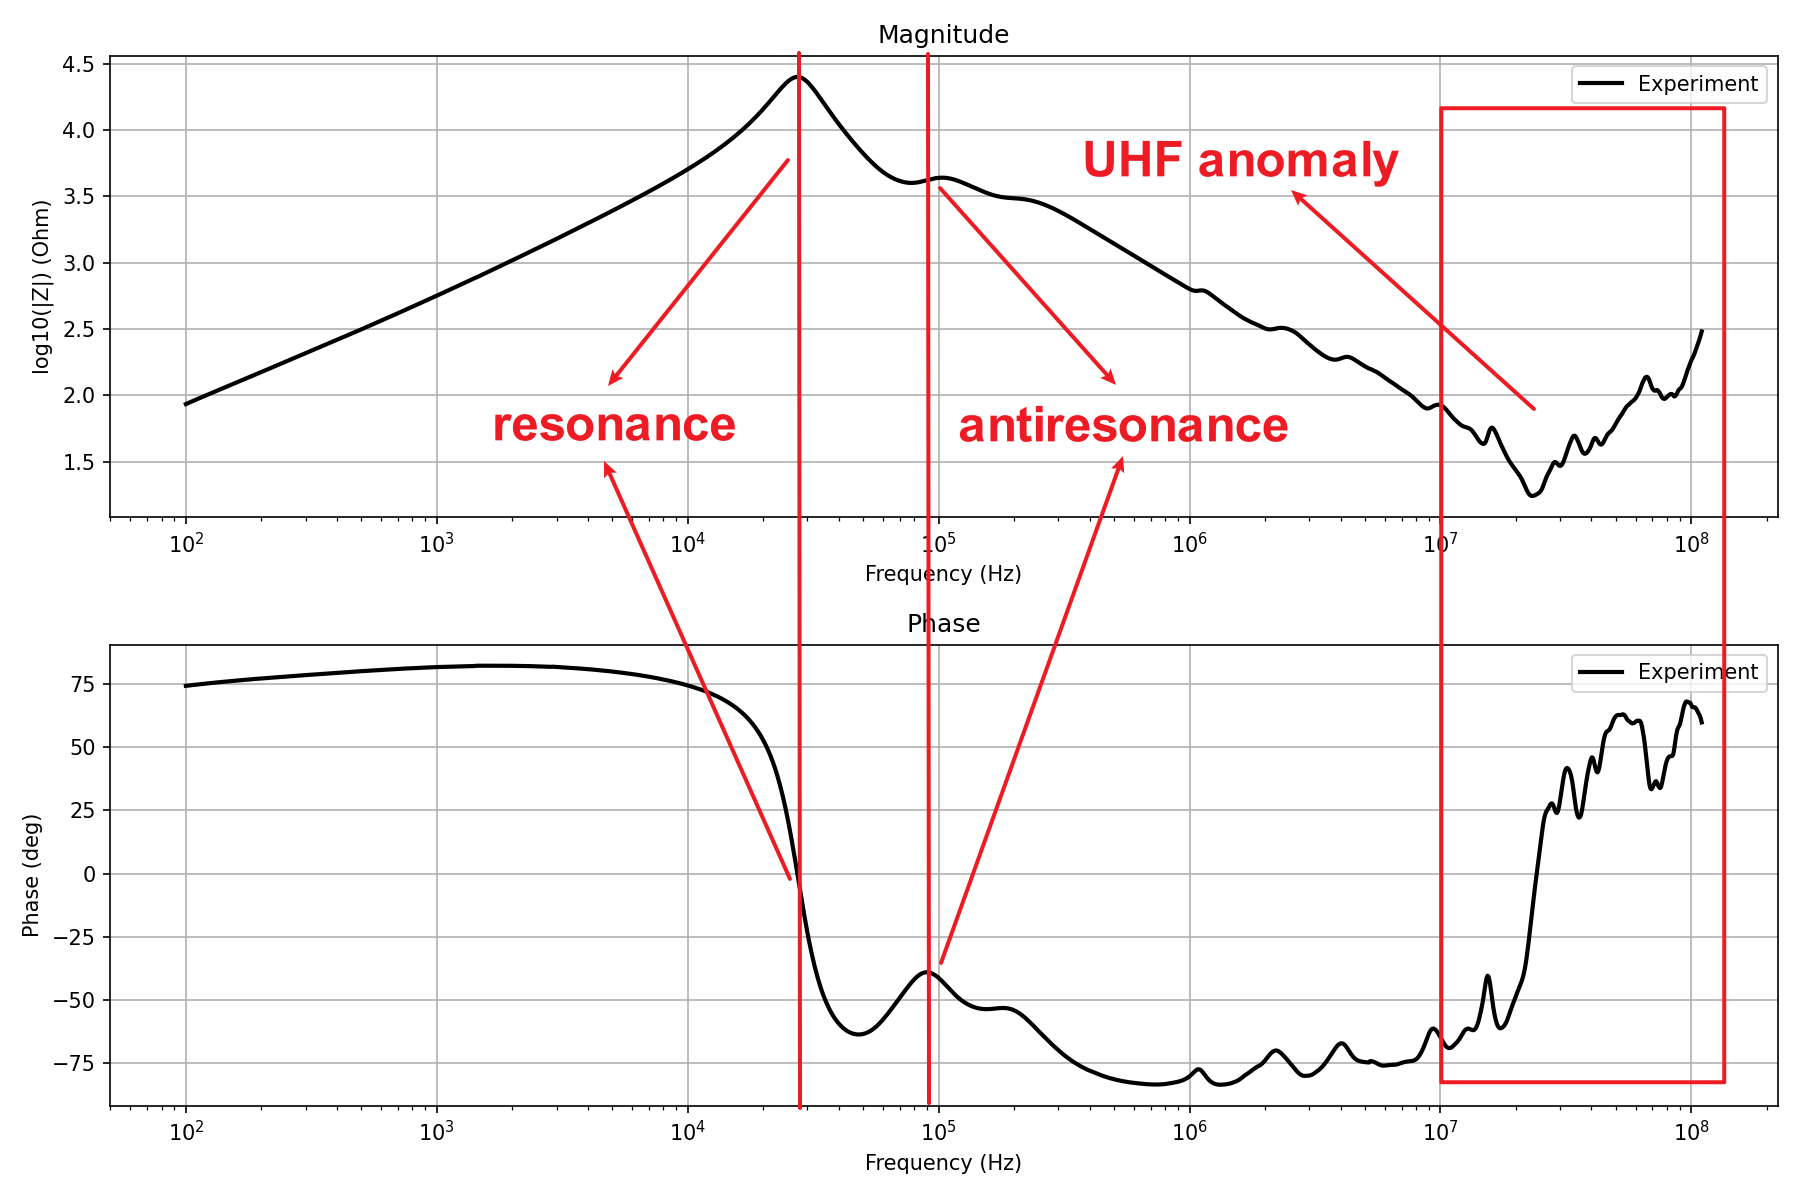
\includegraphics[width=0.82\linewidth]{Add1.png}
    \caption{Measured wideband motor terminal impedance spectrum ($10^2$--$10^8$ Hz) exhibiting characteristic mid-frequency resonances and the anomalous phase-magnitude recovery in the ultra-high-frequency (UHF) regime. }
    \label{fig:measured_impedance}
\end{figure}

In the data considered in this work, the most critical anomalous impedance features do not primarily occur within the conventional megahertz range, but are shifted further into the $10^{7}$--$10^{8}$~ Hz regime. Specifically, the phase exhibits an abnormal upward turn at ultra-high frequency, while the impedance magnitude shows a reversed rise near the high-frequency end; these two behaviors are difficult to reproduce simultaneously using a traditional baseline grey-box circuit. Through initial replication, parameter scanning, and optimizer-level comparisons, we find that stronger optimization alone does not fundamentally resolve this discrepancy. The baseline model remains valid in the low- and mid-frequency ranges, indicating that the underlying low-frequency parameterization and analytical reduction are not the principal source of failure. The true difficulty emerges in the ultra-high-frequency region, where the mismatch is more consistent with insufficient structural degrees of freedom than with poor numerical fitting\cite{ref7,ref13,ref16,ref21,ref24,ref36,ref40}. 

Accordingly, this project aims to develop and evaluate a reproducible grey-box impedance modeling workflow for induction-machine terminal impedance over the frequency range from $10^2$ to $10^8$~Hz. The main objective is to retain the physical interpretability of conventional grey-box motor models while improving their ability to represent the ultra-high-frequency anomaly observed near $10^{7}$--$10^{8}$~Hz.

The project is organized around three practical tasks. First, measured impedance spectra are processed to extract directly observable features and initialize physically meaningful circuit parameters. Second, a conventional grey-box baseline model is constructed and evaluated to identify its valid frequency range and its failure mode in the ultra-high-frequency region. Third, a port-side high-frequency resonant branch is introduced and assessed through full-band fitting, residual analysis, and ablation studies. The purpose of this report is therefore to document the modeling procedure, explain the design choices, present the validation results, and discuss the limitations of the developed model.

\section{Methodology}

\subsection{Measurement Target and Problem Setup}

The primary objective of this work is the characterization and modeling of the measured motor terminal impedance spectrum, defined by the frequency-dependent magnitude $|Z(j\omega)|$ and phase $\angle Z(j\omega)$. Rather than pursuing a black-box regression, this study aims to construct a physically interpretable grey-box model whose validity extends from the conventional low- and mid-frequency (LF–MF) range into the ultra-high-frequency (UHF) regime of $10^7$–$10^8$ Hz\cite{ref12,ref13,ref16,ref20,ref21,ref23,ref40,ref52}.

The modeling target encompasses three distinct spectral features: the dominant resonance and anti-resonance behaviors within the LF–MF range; the global asymptotic magnitude and phase trends; and, critically, the UHF anomaly observed near the upper boundary of the measured band. This anomaly, characterized by an abnormal phase upward turn and a late-frequency magnitude recovery, represents a significant departure from traditional motor circuit behavior. Consequently, the optimization criterion is not confined to the minimization of aggregate fitting error; instead, it prioritizes the preservation of physical consistency in the LF–MF region while ensuring sufficient structural degrees of freedom to represent UHF dynamics\cite{ref1,ref7,ref34,ref36,ref53}.

To satisfy these requirements, the identification framework must distinguish between parameters based on their observability and physical origin. This necessitates a hierarchical approach, detailed in Section 2.2, which classifies the parameter space into directly observable spectral features, analytically initialized quantities, and weakly identifiable terms refined through constrained optimization.

\subsection{Parameter Identification Workflow}

The identification pipeline is structured as a hierarchical workflow that transitions from raw experimental data to a physically consistent parameter set without necessitating auxiliary machine tests. The process comprises three distinct stages: spectral feature extraction, analytical initialization of parasitic components, and global-to-local optimization\cite{ref12,ref13,ref16,ref20,ref21,ref23,ref40,ref45,ref52}.

\subsubsection{Extraction of Direct Spectral Observables}

The identification process commences with the acquisition of the complex terminal impedance $Z(j\omega) = |Z|(\cos\theta + j \sin\theta)$ across the target frequency envelope. To ensure that extracted features reflect persistent electromagnetic structures rather than measurement artifacts, local smoothing and robustness constraints are applied to the raw data. The extraction then targets three primary categories: reactive plateaus, resonance extrema, and inductive slopes.

\paragraph{Capacitive Plateau Identification}
The equivalent ground capacitance $C_{sf}$ is characterized by analyzing the reactive response in regions where the phase approaches $-90^\circ$\cite{ref1,ref7,ref29,ref32,ref36}. The frequency-dependent capacitance is derived as:
\begin{equation}
C_s = -\frac{1}{2\pi f \text{Im}(Z)}
\end{equation}
Two distinct values are identified through windowed plateau detection: $C_{sf\_LF}$ at the low-frequency limit and $C_{sf\_HF}$ at the high-frequency limit. These quantities are subsequently used to formulate the effective mid-frequency capacitance $C_{sf0}$:
\begin{equation}
C_{sf0} = C_{sf\_LF} - 3C_{sf\_HF}
\end{equation}

\paragraph{Inductive and Topological Feature Extraction}
The total leakage inductance $L_\sigma$ is extracted from the inductive regions of the spectrum where $\theta > 0$. The equivalent inductance is calculated via:
\begin{equation}
L_{eq} = \frac{\text{Im}(Z)}{2\pi f}
\end{equation}
To account for stator-rotor partitioning, $L_\sigma$ is scaled by a topology-dependent constant $k$, where $k = 2/3$ for Y-connected configurations and $k = 2$ for Delta-connected configurations. The baseline stator and rotor leakage terms are then initialized under the assumption of balanced leakage distribution, such that $L_{ls} = L_{lr} = 0.5L_\sigma$.

\paragraph{Resonance and Anti-Resonance Detection}
The global resonance ($f_r$) and anti-resonance ($f_a$) frequencies are identified as the local extrema of the impedance magnitude:
\begin{equation}
f_r = \arg \max |Z|, \quad f_a = \arg \min |Z|
\end{equation}
These frequencies, along with their respective magnitude peaks $|Z|_{max}$ and $|Z|_{anti-r}$, serve as the primary constraints for identifying the high-frequency parasitic branches\cite{ref1,ref7,ref34,ref36}. To ensure physical consistency, the search for $f_a$ is subjected to the constraint $0.25 \le \log_{10}(f_a/f_r) \le 0.55$, ensuring that the anti-resonance is correctly associated with the intended parasitic bypass mechanisms.

The extracted observables described above—comprising $C_{sf\_LF}$, $C_{sf\_HF}$, $L_{ls}$, $L_{lr}$, $f_r$, $f_a$, and the associated impedance extrema—provide the necessary information to proceed to the analytical derivation of the remaining grey-box parameters.

\subsubsection{Analytical Initialization of Parasitic Branches}

To clarify the circuit basis of the analytical initialization procedure, Fig.~\ref{fig:single_phase_uim} illustrates the single-phase construction concept underlying the adopted parameterization framework. Its low-frequency backbone follows the standard IEEE 112 T-equivalent circuit, while the added high-frequency parasitic branches define the structural basis for the closed-form initialization relations introduced below.

\begin{figure}[htbp]
    \centering
    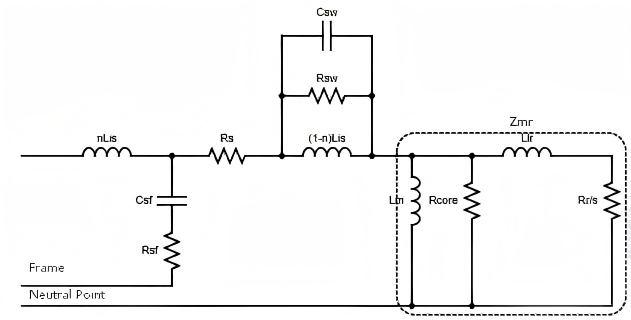
\includegraphics[width=0.82\linewidth]{circuit1p.png}
    \caption{Single-phase equivalent representation of the universal induction motor model, constructed from the standard IEEE 112 T-equivalent backbone with additional high-frequency parasitic branches.}
    \label{fig:single_phase_uim}
\end{figure}

The second stage of the pipeline utilizes the direct observables to initialize high-frequency parasitic parameters through closed-form circuit relations derived from the universal induction motor model topology, following the analytical parameterization framework developed by Mirafzal \textit{et al.}\cite{ref99,ref144}. This analytical step provides a deterministic starting point that reflects the underlying electromagnetic behavior and substantially reduces the search space for subsequent numerical optimization\cite{ref1,ref7,ref12,ref13,ref23,ref40,ref52}.

\paragraph{High-Frequency Reactive Network}
Following the high-frequency branch formulation in the universal induction motor model and its associated parameter-determination procedure\cite{ref99,ref144}, the inter-winding capacitance $C_{sw}$ is initialized from the observed resonance condition, while the additional high-frequency leakage term $\eta L_{ls}$ is inferred from the anti-resonance location. Given the resonance frequency $\omega_r = 2\pi f_r$ and the previously extracted leakage and ground capacitance terms, $C_{sw}$ is initialized for a Y-connected stator as:
\begin{equation}
C_{sw} = \frac{2\omega_r^2 L_{ls} C_{sf} - 1}{\omega_r^2 L_{ls} (\omega_r^2 L_{ls} C_{sf} - 1)}
\end{equation}
In the case of a Delta-connected configuration, the formulation is adjusted by substituting $\omega_r$ with the equivalent frequency term $\omega' = 4\pi f_r$. Concurrently, the additional high-frequency leakage term $\eta L_{ls}$, which governs the location of the anti-resonance point $f_a$, is derived from the reactive balance between the bypass capacitance and the local inductive branch:
\begin{equation}
\eta L_{ls} = \frac{1}{C_{sf} (2\pi f_a)^2}
\end{equation}

\paragraph{Dissipative and Loss Parameters}
The initialization of the dissipative branches likewise follows the parameter-partition strategy reported for the universal induction motor model\cite{ref99,ref144}, where the measured impedance extrema are decomposed into frame-return, inter-winding, and core-loss related contributions. The iron core loss resistance $R_{core}$, which predominantly influences the magnitude in the mid-frequency transition, is estimated using an empirical power-law relation based on the machine’s horsepower ($hp$):
\begin{equation}
R_{core} = 6300 \cdot (hp)^{-0.6958}
\end{equation}
The ground-path loss $R_{sf}$ is initialized from the anti-resonance impedance magnitude as $R_{sf} = (2/3) |Z|_{anti-r}$. For the inter-winding loss $R_{sw}$, which encompasses skin effect and proximity losses at high frequencies, the initialization accounts for the parallel interaction between $R_{core}$ and the inductive reactance $X_L = 2\pi f_r L_{lr}$ at the resonance frequency. The effective value is calculated as:
\begin{equation}
R_{sw} = \frac{2}{3}|Z|_{max} - \frac{R_{core} |X_L|}{\sqrt{R_{core}^2 + X_L^2}}
\end{equation}

This hierarchical initialization ensures that the baseline grey-box model is fully parameterized with values that satisfy the fundamental resonance conditions observed in the measured spectrum before any iterative refinement takes place.

\subsubsection{Optimization and Numerical Refinement}

The final stage of the identification pipeline involves the numerical refinement of the analytically initialized parameter set to minimize the discrepancy between the model response and the experimental observations. To ensure balanced representation across the multi-decade frequency spectrum, the measured data are sampled quasi-uniformly in the $\log_{10} f$ domain before optimization\cite{ref12,ref13,ref38,ref40,ref52}.

\paragraph{Weighted Robust Objective Function}
The optimization target is defined by the joint minimization of the real and imaginary complex impedance residuals. For a parameter vector $\boldsymbol\theta$, the residual components at each frequency point $i$ are formulated as:

\begin{equation}
\begin{aligned}
r_i^{(\text{re})} &= w_i \frac{\text{Re}(Z_i^{\text{sim}}) - \text{Re}(Z_i^{\text{obs}})}{s_{\text{re}}}, \\
r_i^{(\text{im})} &= w_i \frac{\text{Im}(Z_i^{\text{sim}}) - \text{Im}(Z_i^{\text{obs}})}{s_{\text{im}}}
\end{aligned}
\end{equation}

where $s_{\text{re}}$ and $s_{\text{im}}$ are scaling factors estimated via Median Absolute Deviation (MAD) to robustly normalize the error magnitudes and attenuate the influence of outliers. To emphasize structurally significant spectral features, such as resonance transitions and phase reversals, a frequency-dependent weighting scheme $w_i$ is implemented based on the local gradient intensity:

\begin{equation}
\begin{aligned}
\text{score}_i &= \left| \frac{\partial \log |Z|}{\partial \log f} \right|_i + \left| \frac{\partial \angle Z}{\partial \log f} \right|_i, \\
w_i &= \text{clip} \left( \frac{\text{score}_i}{\text{median}(\text{score})}, w_{\min}, w_{\max} \right)
\end{aligned}
\end{equation}

\paragraph{Hybrid Global-to-Local Optimization Strategy}
Numerical stability and the enforcement of parameter positivity are achieved by executing the optimization in the logarithmic parameter space, $u_k = \log \theta_k$. The search strategy combines the explorative capability of Differential Evolution (DE) with the exploitative precision of robust non-linear least squares. The DE algorithm conducts a lightweight global search initialized around the analytical estimates to identify a primary candidate region. Subsequently, a multi-start refinement is performed using boundary-constrained least squares with a robust M-estimator (e.g., soft\_l1 loss) to achieve rapid local convergence while remaining resilient to localized frequency anomalies\cite{ref12,ref13,ref38,ref40,ref52}.

\paragraph{Post-Fit Structural Diagnostic}
Following the optimization, a Gaussian Process (GP) residual analysis is employed to evaluate the structural sufficiency of the identified model. By modeling the remaining residuals as a stochastic process $r(x) \sim \mathcal{GP}(0, k(x, x'))$ using an RBF-plus-noise kernel, the framework distinguishes between random measurement noise and systematic modeling gaps. Significant localized peaks in the predicted GP mean indicate frequency bands where the lumped grey-box topology fails to capture the underlying physics, thereby providing the mechanistic justification for the structural augmentation discussed in the subsequent sections.

\subsection{Baseline Grey-Box Model}

The baseline model utilized in this framework belongs to the class of traditional physically interpretable grey-box formulations. Rather than employing purely mathematical fitting, this approach extends the standard motor equivalent circuit with a localized set of parasitic branches to capture the dominant resonance, anti-resonance, and bypass phenomena observed in wideband terminal measurements\cite{ref12,ref13,ref23,ref40,ref52}.

The circuit topology is partitioned into a low-frequency backbone and a high-frequency parasitic extension. The former comprises the stator and rotor resistances ($R_s, R_r$), leakage inductances ($L_{ls}, L_{lr}$), a magnetizing branch, and core-loss resistance ($R_{core}$), thereby ensuring consistency with classical machine theory in the low- and mid-frequency (LF–MF) ranges. Conversely, the high-frequency extension incorporates winding-to-frame and inter-turn capacitive paths ($C_{sf}, C_{sw}$), leakage partitioning coefficients ($\eta$), and dissipative terms ($R_{sf}, R_{sw}$). These branch parameters are directly mapped to the spectrum-derived observables and analytically initialized quantities established in Section 2.2, maintaining a physically grounded model structure.

The corresponding three-phase baseline topology is shown in Fig.~\ref{fig:baseline_greybox}, where the low-frequency machine backbone is retained and extended by the conventional high-frequency parasitic branches used in structured grey-box modeling.

\begin{figure}[htbp]
    \centering
    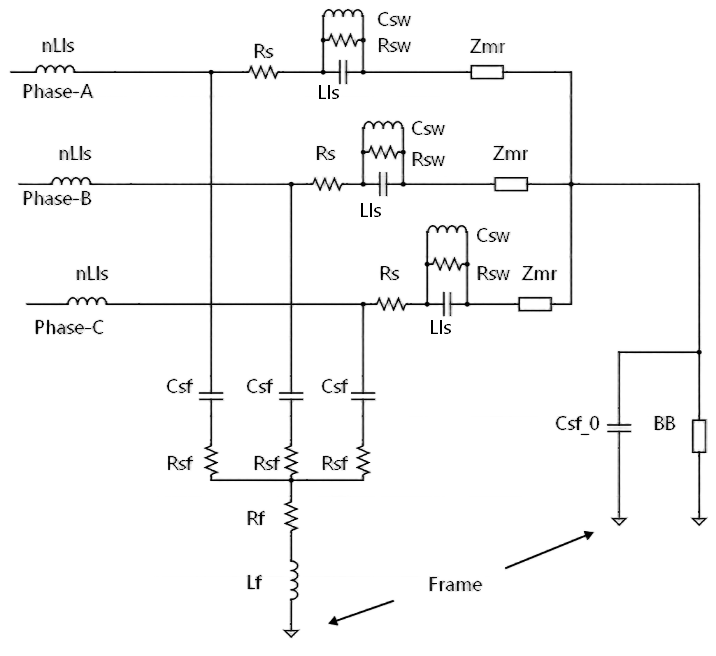
\includegraphics[width=0.82\linewidth]{circuit3p_1.png}
    \caption{Traditional three-phase grey-box equivalent circuit used as the baseline model.}
    \label{fig:baseline_greybox}
\end{figure}

To facilitate efficient numerical refinement, the baseline network is reduced to an analytically sweepable terminal impedance expression through structured equivalent transformations, such as Y-$\Delta$ and series-parallel reductions. This analytical tractability enables rapid evaluation of the full-band frequency response within the optimization loop, significantly mitigating the computational overhead of the "global-to-local" search strategy. 

Despite the effectiveness of this formulation in parameterizing LF–MF characteristics, it remains to be determined whether such a conventional structure possesses sufficient degrees of freedom to replicate the anomalous phase and magnitude transitions observed in the $10^7$–$10^8$ Hz regime. This limitation necessitates the subsequent ultra-high-frequency failure analysis and model augmentation discussed in the following section.

The identified spectral observables, baseline machine parameters, and extracted high-frequency parasitic components for a representative motor instance are consolidated in Table~\ref{tab:parameter_summary_final}. This consolidated parameter set serves as the foundational input for the subsequent circuit formulation and ultra-high-frequency structural analysis.

\begin{table}[htbp]
\caption{Summary of Model Parameters and Identification Methodologies}
\label{tab:parameter_summary_final}
\centering
\begin{tabularx}{\columnwidth}{@{}l>{\raggedright\arraybackslash}X>{\raggedright\arraybackslash}X@{}}
\toprule
\textbf{Symbol} & \textbf{Physical Significance} & \textbf{Identification Method} \\ \midrule
$f_r, f_a$ & Resonance and anti-resonance frequencies & Impedance curve extraction \\
$|Z|_{max}, |Z|_{a}$ & Peak and minimum impedance magnitudes & Impedance curve extraction \\ \midrule
$L_{ls}, L_{lr}$ & Stator and rotor leakage inductances & Impedance curve approximation \\
$R_{core}$ & Core loss equivalent resistance & Empirical formula \\
$R_s, R_r/s$ & Stator and rotor resistance components & Impedance curve approximation \\ \midrule
$C_{sf}$ & Stator-to-frame capacitance (boundary limits) & Impedance curve approximation \\
$C_{sf0}$ & Effective mid-frequency ground capacitance & Analytical derivation \\
$C_{sw}$ & Inter-winding stray capacitance & Analytical derivation \\
$\eta L_{ls}$ & High-frequency effective leakage term & Analytical derivation \\
$R_{sw}, R_{sf}$ & Parasitic and frame-return loss terms & Analytical derivation \\ \bottomrule
\end{tabularx}
\end{table}

\section{Model Analysis and Improvement}

\subsection{Baseline Model Performance}

This subsection evaluates the conventional grey-box baseline defined in Section 2 on the measured terminal impedance spectra. 

Validation is assessed primarily over the frequency range in which the physical assumptions of the baseline are expected to remain meaningful. In this subsection, a successful validation does not imply a perfect full-band fit. It requires that the model reproduce the dominant resonance and antiresonance structure in the low- and mid-frequency range, preserve the main magnitude and phase trends, and remain consistent with the characteristic frequencies and plateau-derived quantities extracted from the measured spectra. Under this criterion, agreement in the conventional range is sufficient to support the credibility of the baseline parameterization and analytical circuit backbone.

The measured-versus-baseline impedance curves show that this requirement is met in the low- and mid-frequency regime. The baseline captures the dominant spectral trend, reproduces the principal resonance and antiresonance locations with reasonable fidelity, and yields a magnitude/phase evolution that remains consistent with the measured response over the conventional range. This result indicates that the extracted parameters and the analytical reduction are not arbitrary numerical constructs, but form a physically meaningful representation of the terminal impedance before the onset of the ultra-high-frequency anomaly.

A clear mismatch emerges, however, when the anomalous behavior shifts into the $10^{7}$--$10^{8}$~ Hz regime. In this region, the measured late-frequency magnitude recovery is weakened or absent in the baseline response, and the abnormal phase rise is not reproduced with comparable fidelity. The deviation is systematic rather than a localized fluctuation, which suggests that the issue cannot be reduced to random measurement noise\cite{ref7,ref13,ref16,ref21,ref24,ref36,ref40}. This observation motivates the failure analysis in the next subsection.

\subsection{Failure Mechanism in the Ultra-High-Frequency Range}

\subsubsection{Dominant-path analysis in the UHF regime}

The frequency-localized nature of the baseline limitation is illustrated in Fig.~\ref{fig:baseline_band_comparison}. The model remains reasonably consistent with the measured response before the UHF tail, while the mismatch becomes pronounced in the $10^{7}$--$10^{8}$~Hz range.

\begin{figure}[htbp]
    \centering
    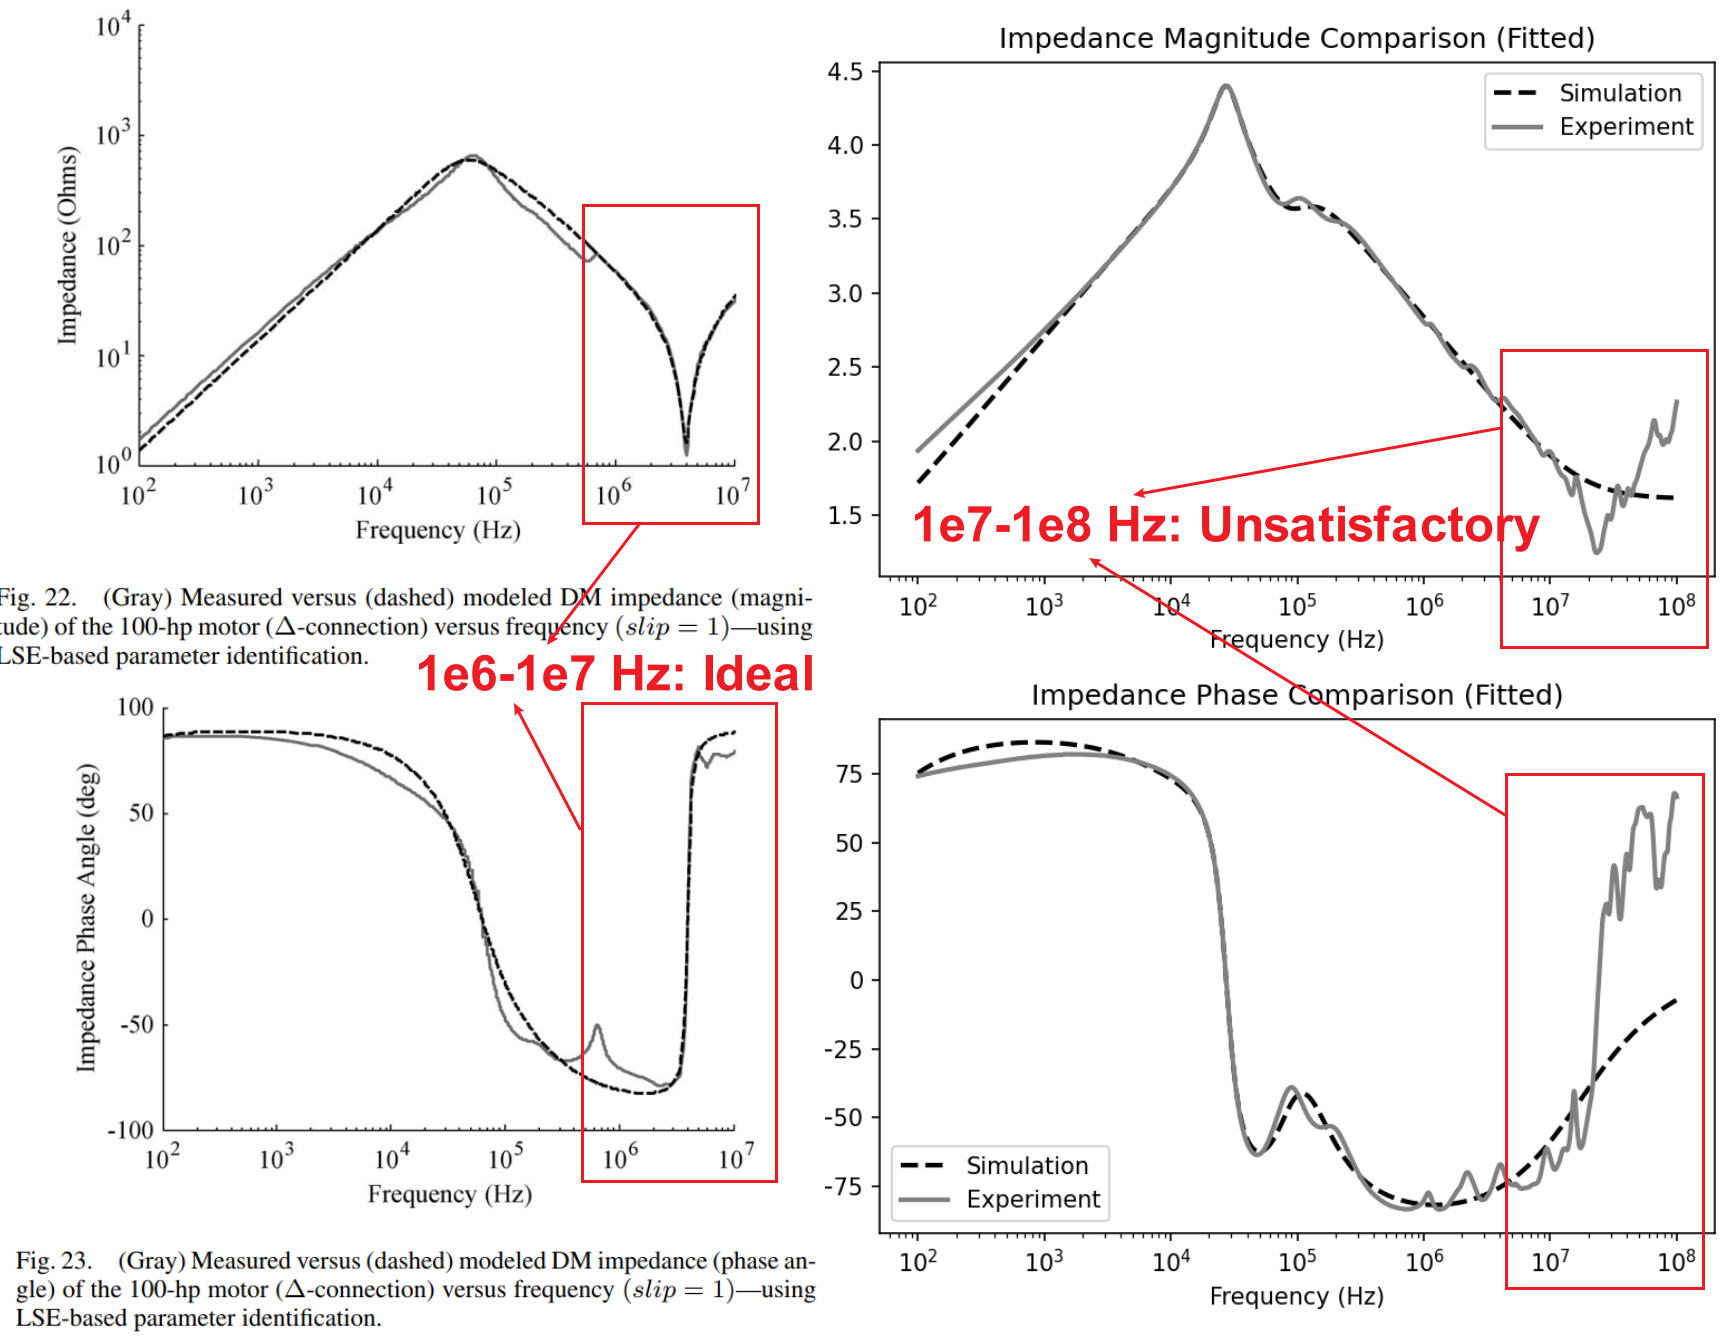
\includegraphics[width=0.82\linewidth]{Add4.png}
    \caption{Baseline-model fitting behavior in different high-frequency regions. The conventional grey-box model remains effective up to the $10^{6}$--$10^{7}$~Hz range but becomes insufficient in the $10^{7}$--$10^{8}$~Hz UHF region, especially in reproducing the phase rise and magnitude recovery.}
    \label{fig:baseline_band_comparison}
\end{figure}

To diagnose the failure of the conventional grey-box baseline in the $10^{7}$--$10^{8}$~ Hz range, the analytical focus must shift from terminal mismatch to internal branch composition. The fundamental inquiry is whether inductive components retain control over the terminal response as the branch hierarchy evolves at ultra-high frequencies (UHF).

Structural analysis is performed on a star (short) DM\&CM configuration, where the input network is decomposed into several physically distinct blocks:

\begin{itemize}[leftmargin=*, itemsep=0pt]
    \item \textbf{$Z_{\text{mr}}$}: The magnetizing-rotor block (rotor branch, core-loss resistance, and magnetizing inductance in parallel).
    \item \textbf{$Z_{\text{mid}}$}: The stator internal path (stator resistance in series with an RLC leakage/inter-turn subnetwork).
    \item \textbf{$Z_{\text{nLls}}$}: Fractional stator leakage inductance.
    \item \textbf{$Z_{\text{bra}}, Z_{\text{csf0}}$}: The stator-to-frame and equivalent stator stray-capacitance branches, respectively.
\end{itemize}

These elements are integrated into a topology-consistent terminal impedance, $Z_{\text{total}}$, through successive Y-Delta transformations and series-parallel reductions. This framework reveals a frequency-dependent inversion of branch dominance. At 100~Hz, the response is governed by the motor backbone ($|Z_{\text{mr}}| = 13.0~\Omega$; $|Z_{\text{mid}}| = 22.4~\Omega$), while the high-frequency return and bypass paths remain effectively open ($|Z_{\text{bra}}| = 4.60 \times 10^6~\Omega$; $|Z_{\text{csf0}}| = 2.16 \times 10^5~\Omega$). However, at 110~MHz, this hierarchy reverses: $|Z_{\text{csf0}}|$ drops to 0.196~$\Omega$, whereas $|Z_{\text{mr}}|$ rises to 5265~$\Omega$. Consequently, the UHF terminal response is no longer determined by the conventional motor branches but is instead dominated by low-impedance capacitive bypass paths.

Fig.~\ref{fig:uhf_tail_conditions} summarizes the measured UHF tail behavior under several wiring configurations. The repeated pattern provides practical motivation for treating the high-frequency tail as a boundary-aware terminal modeling issue.

\begin{figure}[htbp]
    \centering
    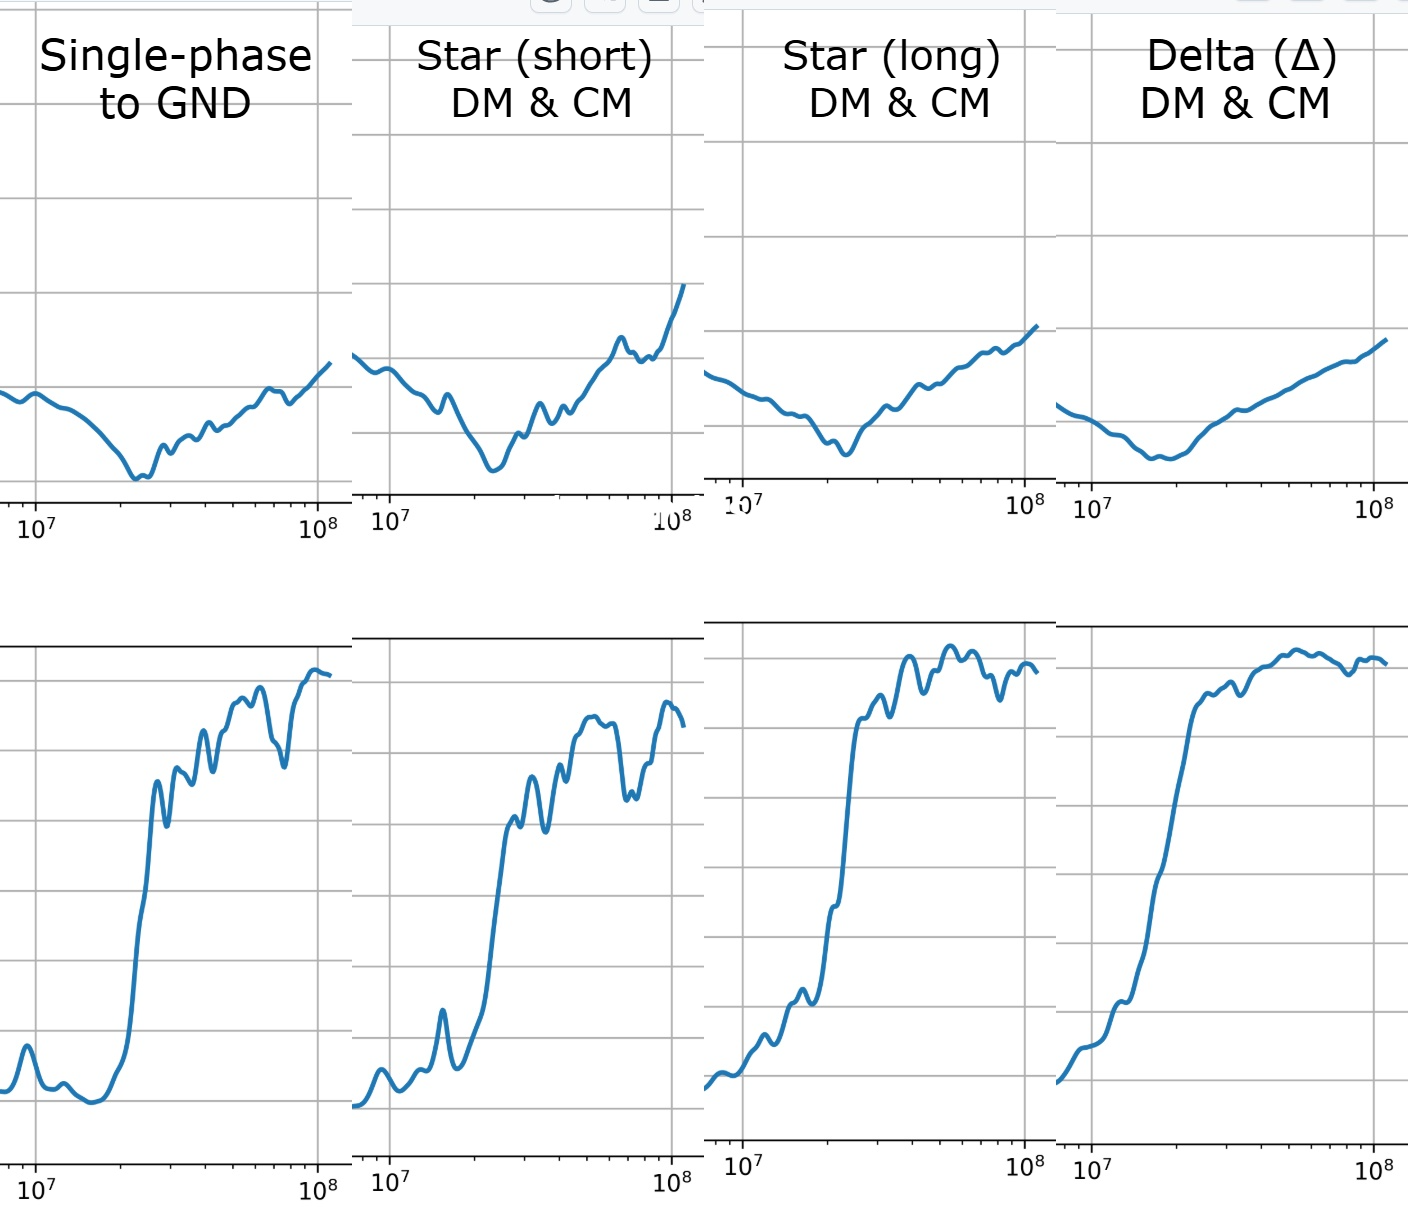
\includegraphics[width=0.82\linewidth]{Add3.png}
    \caption{Comparison of the ultra-high-frequency impedance-tail behavior under different measurement configurations, including single-phase-to-ground, star-connected, and delta-connected conditions. The repeated phase-rise and magnitude-recovery pattern suggests that the UHF response is strongly influenced by the measurement boundary and return-path condition.}
    \label{fig:uhf_tail_conditions}
\end{figure}

\subsubsection{Structural insensitivity of the baseline formulation}

The dominance of bypass paths does not imply the disappearance of inductive contributions. On the contrary, the inductive branch $|Z_{\text{nLls}}|$ increases from $1.12 \times 10^{-6}~\Omega$ at 100~Hz to 1.23~$\Omega$ at 110~MHz, maintaining a phase near $+90^\circ$. The failure of the baseline model arises because these inductive terms cannot emerge as the controlling branches at the terminal level. Once the lower-impedance bypass paths dominate the network, local inductive tendencies are effectively masked within the combined output.

\begin{figure}[htbp]
    \centering
    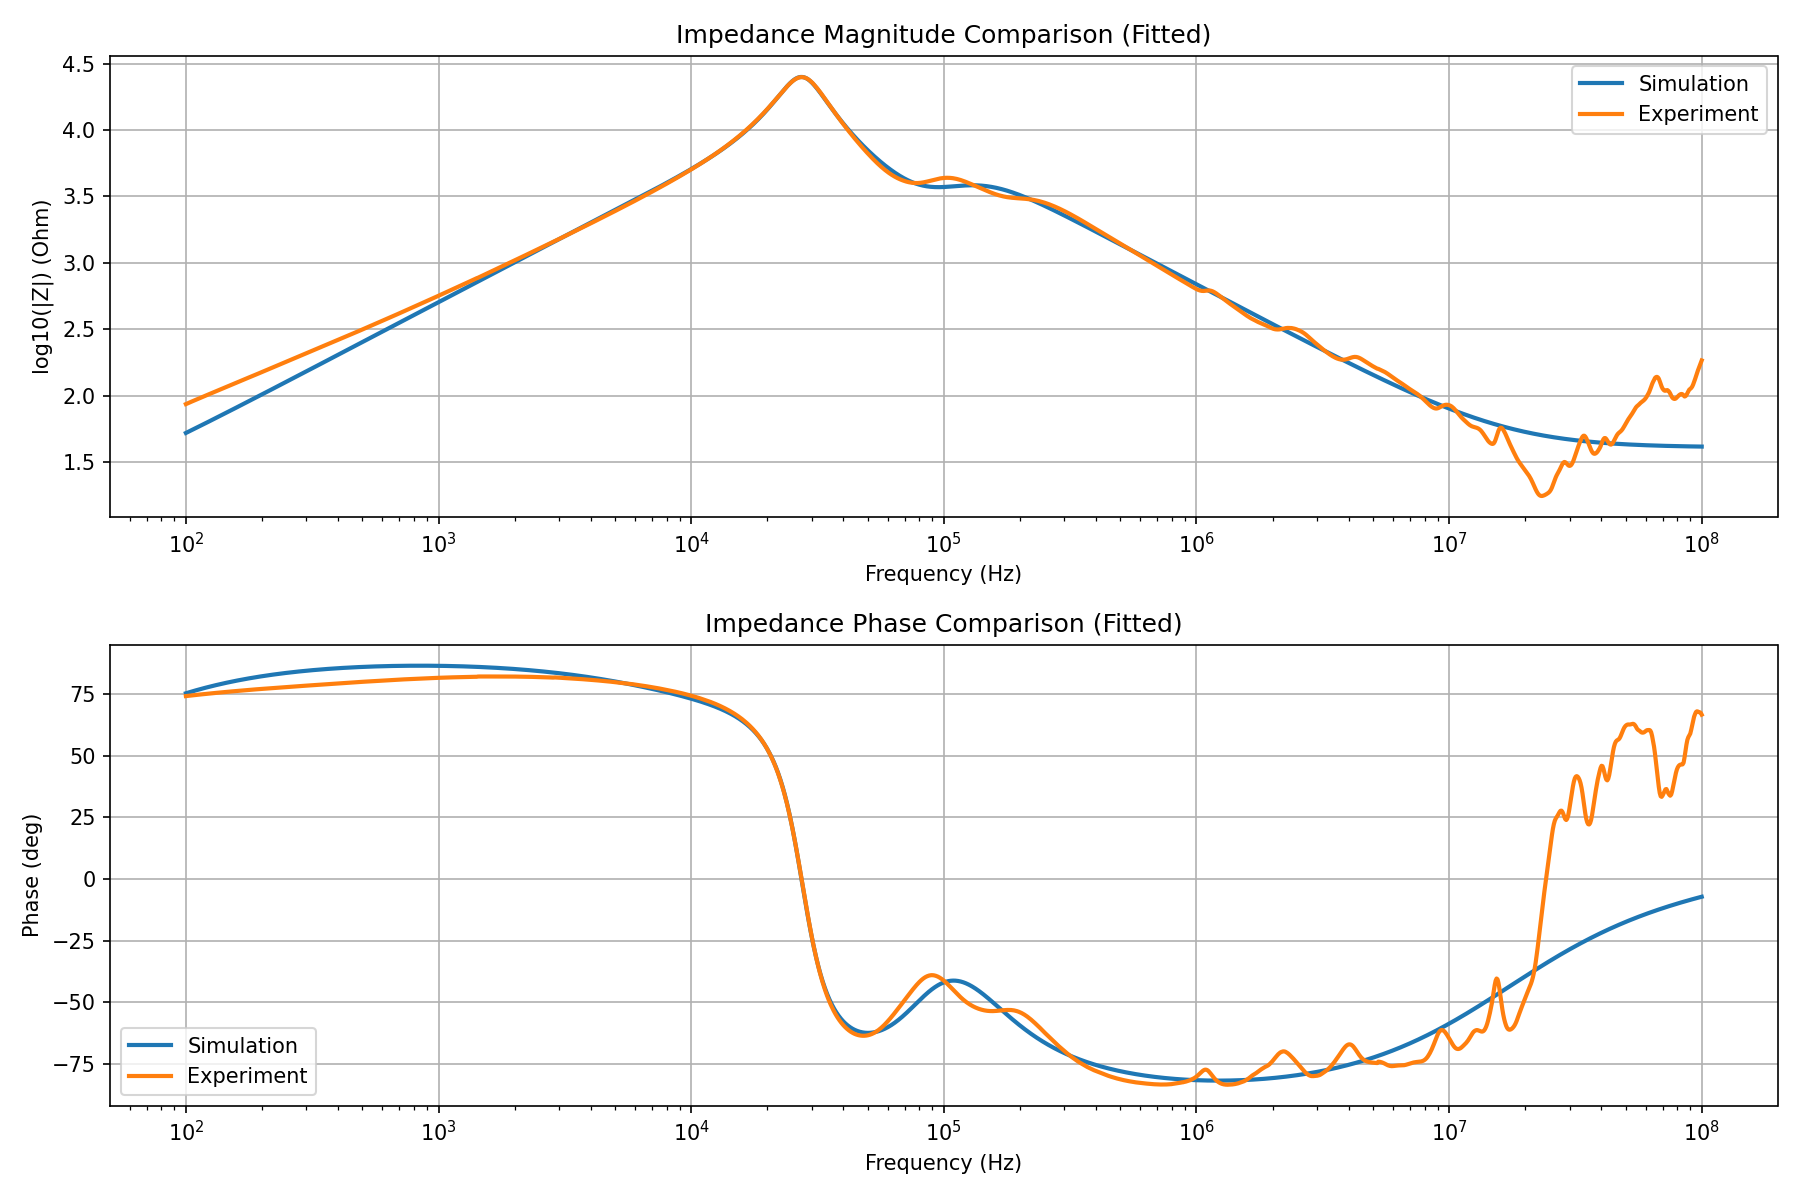
\includegraphics[width=0.82\linewidth]{fig_noL.png}
    \caption{Fitting performance of the baseline model without the port-side resonant augmentation. While the model provides reasonable agreement in the low- and mid-frequency regions, it fails to capture the anomalous behavior in the ultra-high-frequency (UHF) range, particularly in the phase response.}
    \label{fig:baseline_fit}
\end{figure}

\begin{figure}[htbp]
    \centering
    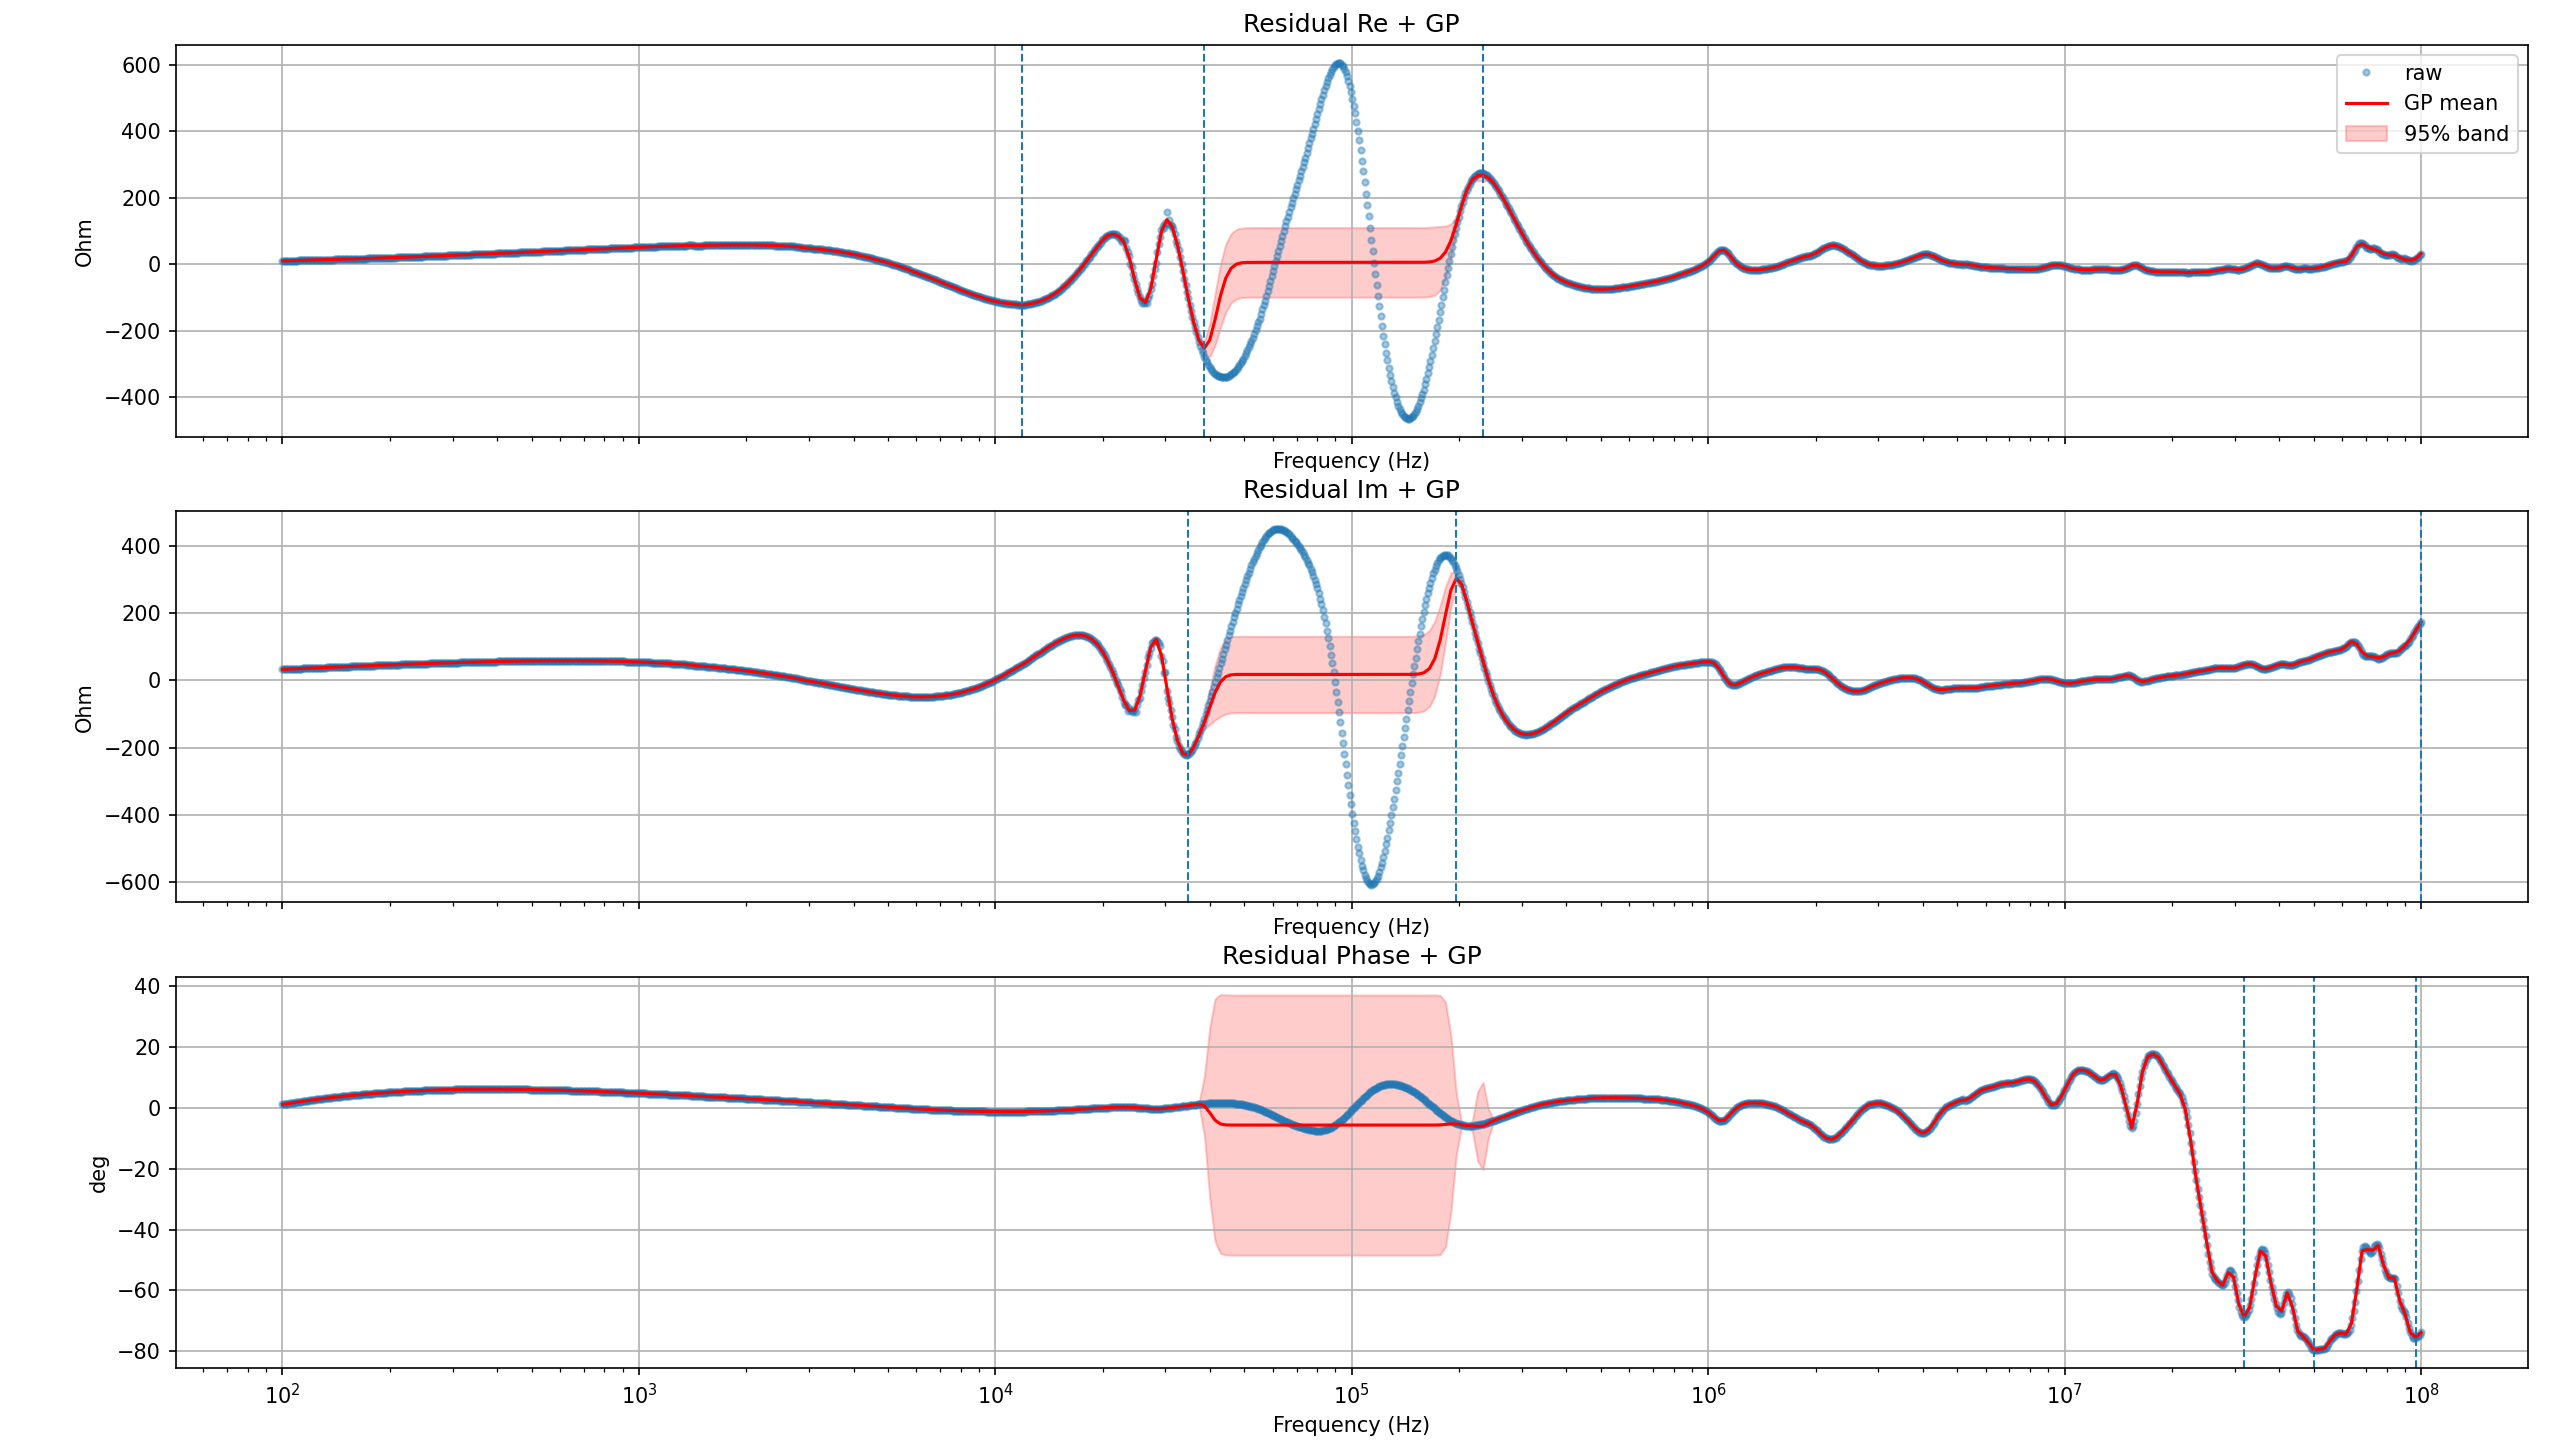
\includegraphics[width=0.82\linewidth]{fig_noL_gp.png}
    \caption{Residual structure of the baseline model in real, imaginary, and phase components. The presence of coherent residual patterns across multiple frequency bands confirms that the model error is structural in nature, rather than arising from suboptimal parameter estimation.}
    \label{fig:baseline_residual}
\end{figure}

This masking effect explains the observed "structural insensitivity" of the baseline formulation. If the mismatch were merely a result of inaccurate parameterization, local adjustments to inductive values would significantly alter the terminal behavior. Instead, the UHF response remains largely unresponsive to such variations, indicating that the dominant bypass paths and the rigid baseline topology jointly "lock" the terminal output. Therefore, the failure of the baseline in the $10^{7}$--$10^{8}$~ Hz range represents a fundamental structural limitation: while inductive components are present, they are prevented from shaping the terminal-level phase rise or magnitude recovery due to the existing branch competition.

\subsection{Port-Side High-Frequency Model Improvement}

The diagnostic analysis in Section 3.2 establishes that the ultra-high-frequency (UHF) mismatch originates from the topological saturation of the baseline network. In the $10^7$–$10^8$ Hz regime, the terminal response is governed by a restricted subset of low-impedance capacitive bypass paths, rendering the terminal impedance largely insensitive to the adjustment of internal motor branches\cite{ref8,ref16,ref20,ref21,ref24,ref45}. To restore the necessary modeling expressiveness, an auxiliary high-frequency degree of freedom is introduced directly at the measurement port.

The experimental impedance spectra exhibit a distinct transition from capacitive to inductive behavior within the target $10^7$–$10^8$ Hz range, characterized by non-monotonic phase reversals and high-frequency oscillations. Such features are characteristic of distributed parasitic effects rather than the lumped parameter dynamics of the internal motor core. An order-of-magnitude estimation reveals that for an equivalent ground capacitance in the nanofarad ($nF$) range—typical for stator-to-frame paths—a series parasitic inductance of only tens of nanohenries ($nH$) is sufficient to trigger a phase reversal in the 10–100 MHz band. This level of inductance is consistent with the equivalent series inductance (ESL) of large capacitive components, terminal leads, or the geometric loop formed by the machine enclosure and the grounding system.

Consequently, the failure of the baseline model is not a result of insufficient optimization of internal branches, such as the stator leakage or magnetizing sub-networks, but rather the absence of a dedicated port-side inductive mechanism. The proposed augmentation is thus formulated as a damped resonant cell consisting of a parallel $L_{ad} || C_{ad}$ combination in series with a damping resistance $R_{ad}$. From a network synthesis perspective, this structure introduces a localized pole-zero pair that enables frequency-selective shaping of the impedance trajectory. While $L_{ad}$ provides the necessary inductive lift to reproduce the phase upward turn, the inclusion of $C_{ad}$ and $R_{ad}$ ensures that the model can capture the structured magnitude recovery and localized oscillations without inducing unrealistic, undamped peaks. The resulting augmented three-phase topology is shown in Fig.~\ref{fig:augmented_model}, where the practically negligible $R_f$--$L_f$ frame-return branch is removed to decouple the network phases and facilitate subsequent circuit derivations.

\begin{figure}[htbp]
    \centering
    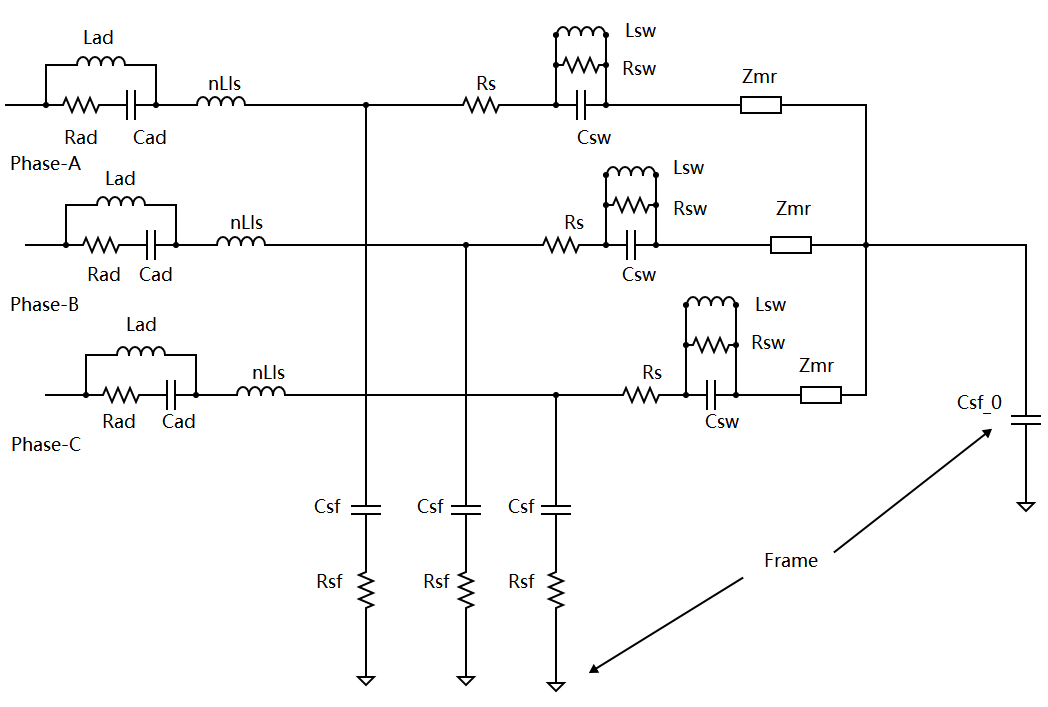
\includegraphics[width=0.82\linewidth]{circuit3p_2.png}
    \caption{Proposed augmented three-phase grey-box model with a port-side resonant cell and simplified frame-return path.}
    \label{fig:augmented_model}
\end{figure}

\section{Results and Discussion}

\subsection{Evaluation Criteria}

The experimental evaluation substantiates the modeling efficacy of the proposed framework through comparative benchmarks against the measured motor terminal impedance ($10^2$--$10^8$ Hz). To ensure statistical rigor, all compared methods utilize identical parameter bounds and circuit topologies, ensuring that performance variations are strictly attributable to the model structure and optimization strategy . 

The performance is quantified across three dimensions:

\paragraph{Fitting Accuracy and Information Criteria}
To ensure physical interpretability, accuracy is primarily evaluated in the raw complex impedance space using the Root Mean Squared Error ($RMSE_{\text{raw}}$). To further account for the wide dynamic range of impedance magnitudes across six decades, a magnitude-based relative metric is introduced. The relative magnitude error is defined as $e_{i,\text{mag}} = (|Z_i^{\text{sim}}| - |Z_i^{\text{obs}}|) / |Z_i^{\text{obs}}|$, providing a frequency-independent assessment of modeling fidelity across the spectrum. The resulting $RMSE_{\text{rel}}$ represents the average percentage deviation of the model magnitude from the measured data. 

Furthermore, to balance accuracy with model complexity, the Akaike and Bayesian Information Criteria (AIC and BIC) are calculated in the raw impedance space. These criteria statistically justify the structural augmentation in the UHF regime by ensuring that the improvement in likelihood outweighs the addition of parasitic parameters.

\paragraph{Computational Complexity and Robustness}
Algorithm efficiency is assessed via the total number of model evaluations ($N_{\text{eval}}$) and execution time, providing a platform-independent view of search complexity . Given the stochastic nature of global optimizers, robustness is evaluated through 10 independent trials per configuration, with results reported as mean $\pm$ standard deviation to distinguish average fitting quality from numerical stability .

\paragraph{Structural Diagnostics}
A Gaussian Process (GP) regression is applied to the post-fit residuals as a posterior diagnostic tool. The residual $r(x)$ at a standardized logarithmic frequency $x = \log_{10}f$ is modeled as:
\begin{equation}
r(x) \sim \mathcal{GP}(0, k(x, x'))
\end{equation}
where the kernel $k(x, x')$ combines a Radial Basis Function (RBF) with a white noise term to decouple random measurement noise from systematic modeling gaps . Significant peaks in the predicted mean $|\mu(x)|$ serve to localize frequency bands where the lumped grey-box topology fails to capture the underlying physics .

\subsection{Main Results and Residual Analysis}

\subsubsection{Full-Band Fitting Performance}

The simulated terminal impedance response of the proposed method demonstrates high fidelity to the experimental data across the entire six-decade frequency spectrum. Within the low- and mid-frequency (LF–MF) range, the model accurately replicates the dominant resonance and anti-resonance profiles, with the simulated magnitude and phase trajectories remaining closely aligned with the measured response. This agreement confirms that the hierarchical parameterization established in Section 2 and the underlying grey-box circuit carrier remain valid within the frequency regime where lumped physical assumptions are most prominent.

\begin{table}[htbp]
\caption{Consolidated Performance Metrics and Computational Complexity}
\label{tab:proposed_performance}
\centering
\begin{tabularx}{\columnwidth}{Xcc} % X 表示该列自动填满剩余空间
\hline
\textbf{Metric Description} & \textbf{Raw Value} & \textbf{Rel. / Detail} \\
\hline
Root Mean Squared Error (RMSE) & 130.87 & 0.2164 \\
Sum of Squared Errors (SSE) & $5.447 \times 10^7$ & 74.48 \\
Akaike Information Criterion (AIC) & 31028.04 & -- \\
Bayesian Information Criterion (BIC) & 31112.94 & -- \\
\hline
Total Wall-clock Time ($T_{\text{fit}}$) & \multicolumn{2}{c}{8.399 s} \\
Global/Local Time Split & \multicolumn{2}{c}{1.880 s / 6.321 s} \\
\hline
\end{tabularx}
\end{table}

\begin{figure}[htbp]
    \centering
    \includegraphics[width=0.82\linewidth]{fig_Curver.png}
    \caption{Full-band comparison between the proposed model (CurVer) and experimental measurements for both impedance magnitude and phase over the frequency range $10^2$--$10^8$ Hz. The model accurately captures the mid-frequency resonance behavior as well as the anomalous recovery in the ultra-high-frequency (UHF) regime.}
    \label{fig:curver_fit}
\end{figure}

The enhancement in modeling capability is most evident in the $10^7$–$10^8$ Hz regime, where the proposed method successfully recovers the two characteristic behaviors that motivated this study: the late-frequency magnitude recovery and the phase upward transition observed near the upper measurement boundary. These features emerge as coherent terminal-level responses rather than isolated numerical corrections, indicating that the introduction of the port-side high-frequency degree of freedom effectively extends the model's expressive range without compromising its consistency in the conventional frequency bands.

Quantitative error metrics are consistent with these visual observations. For the representative full-band case, the proposed framework achieves a raw-space Sum of Squared Errors ($SSE_{raw}$) of $5.44654 \times 10^7$ and a Root Mean Squared Error ($RMSE_{raw}$) of $130.872$ across $n = 3180$ residual dimensions. The associated information criteria, $AIC_{raw} = 31028.036$ and $BIC_{raw} = 31112.941$, provide a standardized reference for assessing the trade-off between model complexity and fitting accuracy. These metrics demonstrate that the model attains superior numerical accuracy while preserving the primary physical structures of the motor impedance within a unified formulation. Consequently, the principal contribution of the proposed methodology is not merely a reduction in aggregate error, but the realization of a full-band response that maintains structural integrity in the conventional regime and substantial expressiveness in the ultra-high-frequency boundary regime.

\subsubsection{Residual-Structure Diagnosis}

The Gaussian Process (GP) regression serves as a posterior diagnostic tool to localize unresolved structural mismatches within the frequency domain. As shown in the residual manifold, the modeling error is concentrated in discrete frequency bands rather than being uniformly distributed, providing a mechanistic map of the model's structural limits.For the real and imaginary components, the dominant residual structures are primarily localized within the $10^4$–$10^5$ Hz range, coinciding with the primary resonance and anti-resonance neighborhood. Specifically, the GP mean for the real part exhibits peaks at $1.19 \times 10^4$ Hz, $3.86 \times 10^4$ Hz, and $2.34 \times 10^5$ Hz, while the imaginary part shows significant mismatches at $3.48 \times 10^4$ Hz, $1.96 \times 10^5$ Hz, and $3.08 \times 10^5$ Hz. These deviations suggest that while the baseline motor core captures the fundamental machine dynamics, minor refinements in the mid-band lumped parameterization could further mitigate the localized structural residual.

\begin{figure}[htbp]
    \centering
    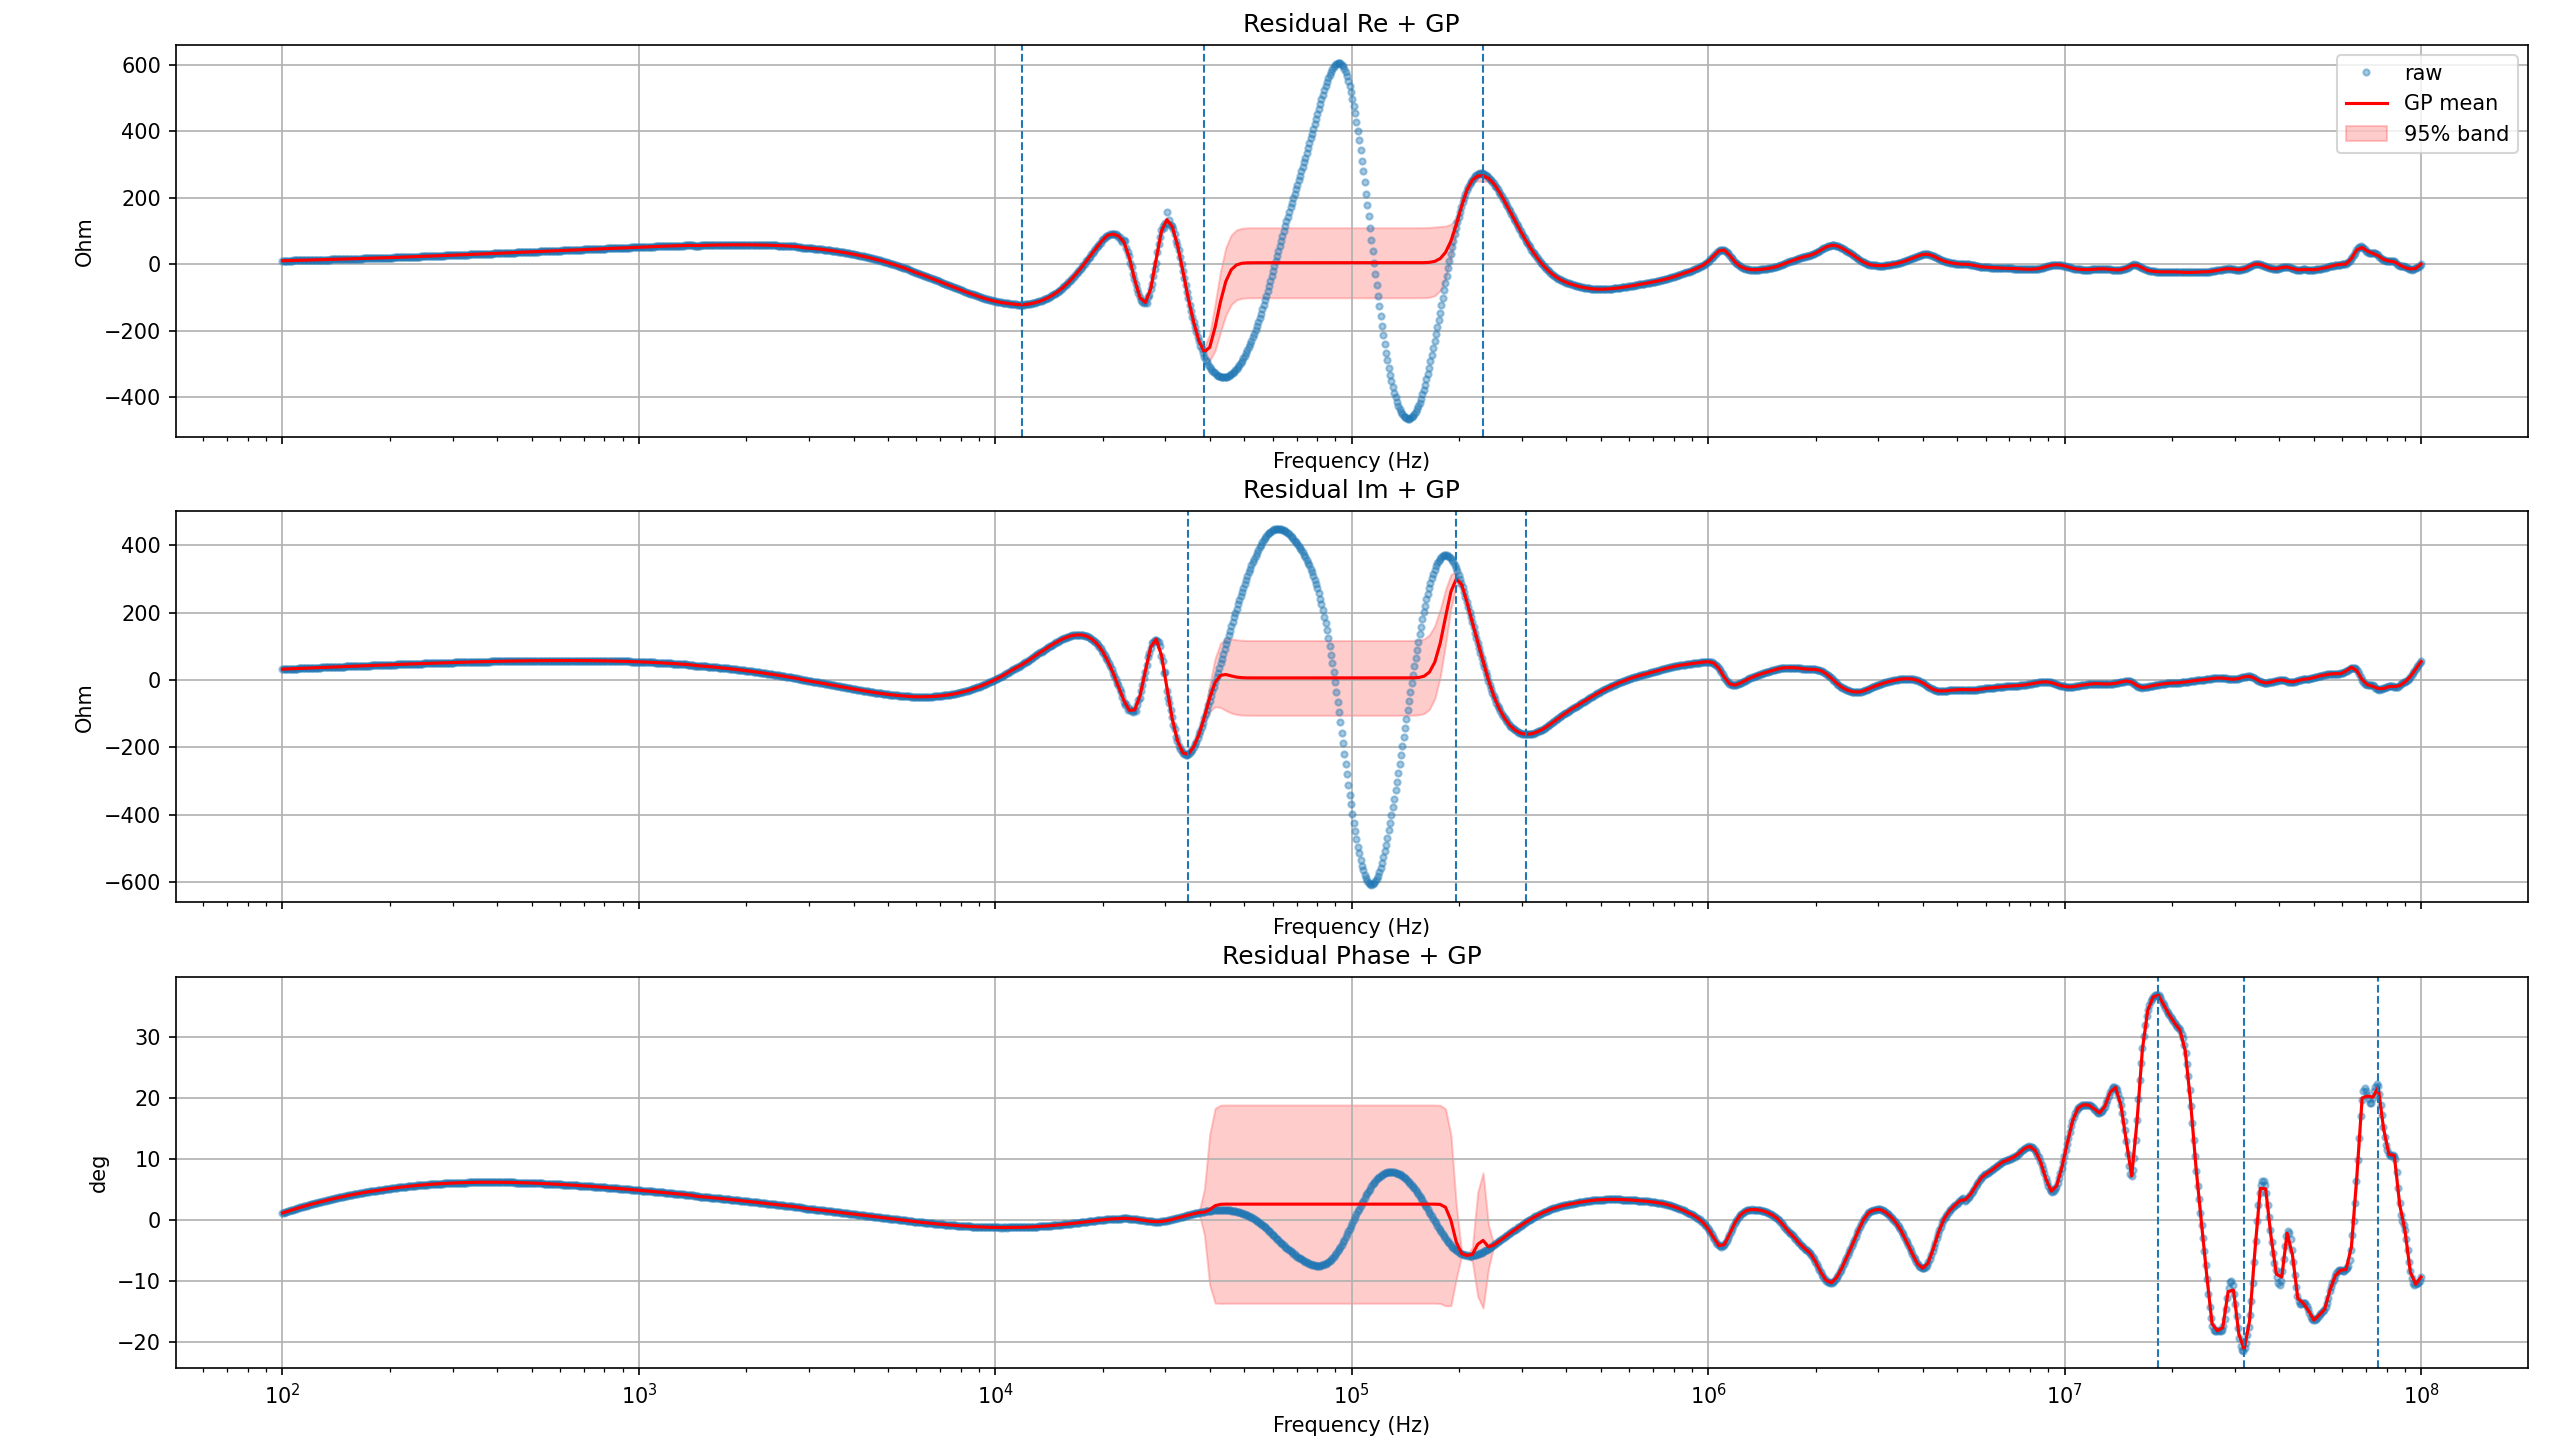
\includegraphics[width=0.82\linewidth]{fig_curver_gp.png}
    \caption{Residual structure of the CurVer model in real, imaginary, and phase components, with Gaussian process (GP) regression. Structured deviations are observed in specific frequency bands, particularly in the UHF region, indicating that the remaining mismatch is systematic and linked to model structure rather than optimization limitations.}
    \label{fig:curver_residual}
\end{figure}

In contrast, the phase residual peaks are significantly shifted toward the target ultra-high-frequency (UHF) regime, with dominant structures identified at $1.83 \times 10^7$ Hz, $3.19 \times 10^7$ Hz, and $7.58 \times 10^7$ Hz. The remaining phase mismatch is confined to the $10^7$–$10^8$ Hz interval, where the measured response exhibits stochastic irregularities and high-order fluctuations that transcend the deterministic capacity of lumped parameter modeling. In this UHF regime, the observed impedance profiles are characterized by extreme randomness and boundary sensitivity, such that exhaustive structural matching of these localized features would likely lead to over-fitting rather than an improved physical representation. Consequently, the GP analysis confirms that the primary modeling limitations are restricted to non-systemic high-frequency dynamics, rendering the current residual level an acceptable and anticipated result of the grey-box formulation.

\subsubsection{Optimization-side sanity check}
To distinguish structural limitations from optimization deficiencies, an additional sanity check is conducted by comparing the deterministic least-squares (LS) solution against a Bayesian reference generated via the No-U-Turn Sampler (NUTS). The resulting Maximum A Posteriori (MAP) and LS responses remain congruent across the full frequency band, preserving identical resonance structures in the low- and mid-frequency (LF–MF) ranges. In the ultra-high-frequency (UHF) regime, the posterior mean exhibits localized smoothing relative to the MAP result, a behavior characteristic of posterior averaging in weakly constrained subspaces rather than the discovery of a distinct optimum.

\begin{figure}[htbp]
    \centering
    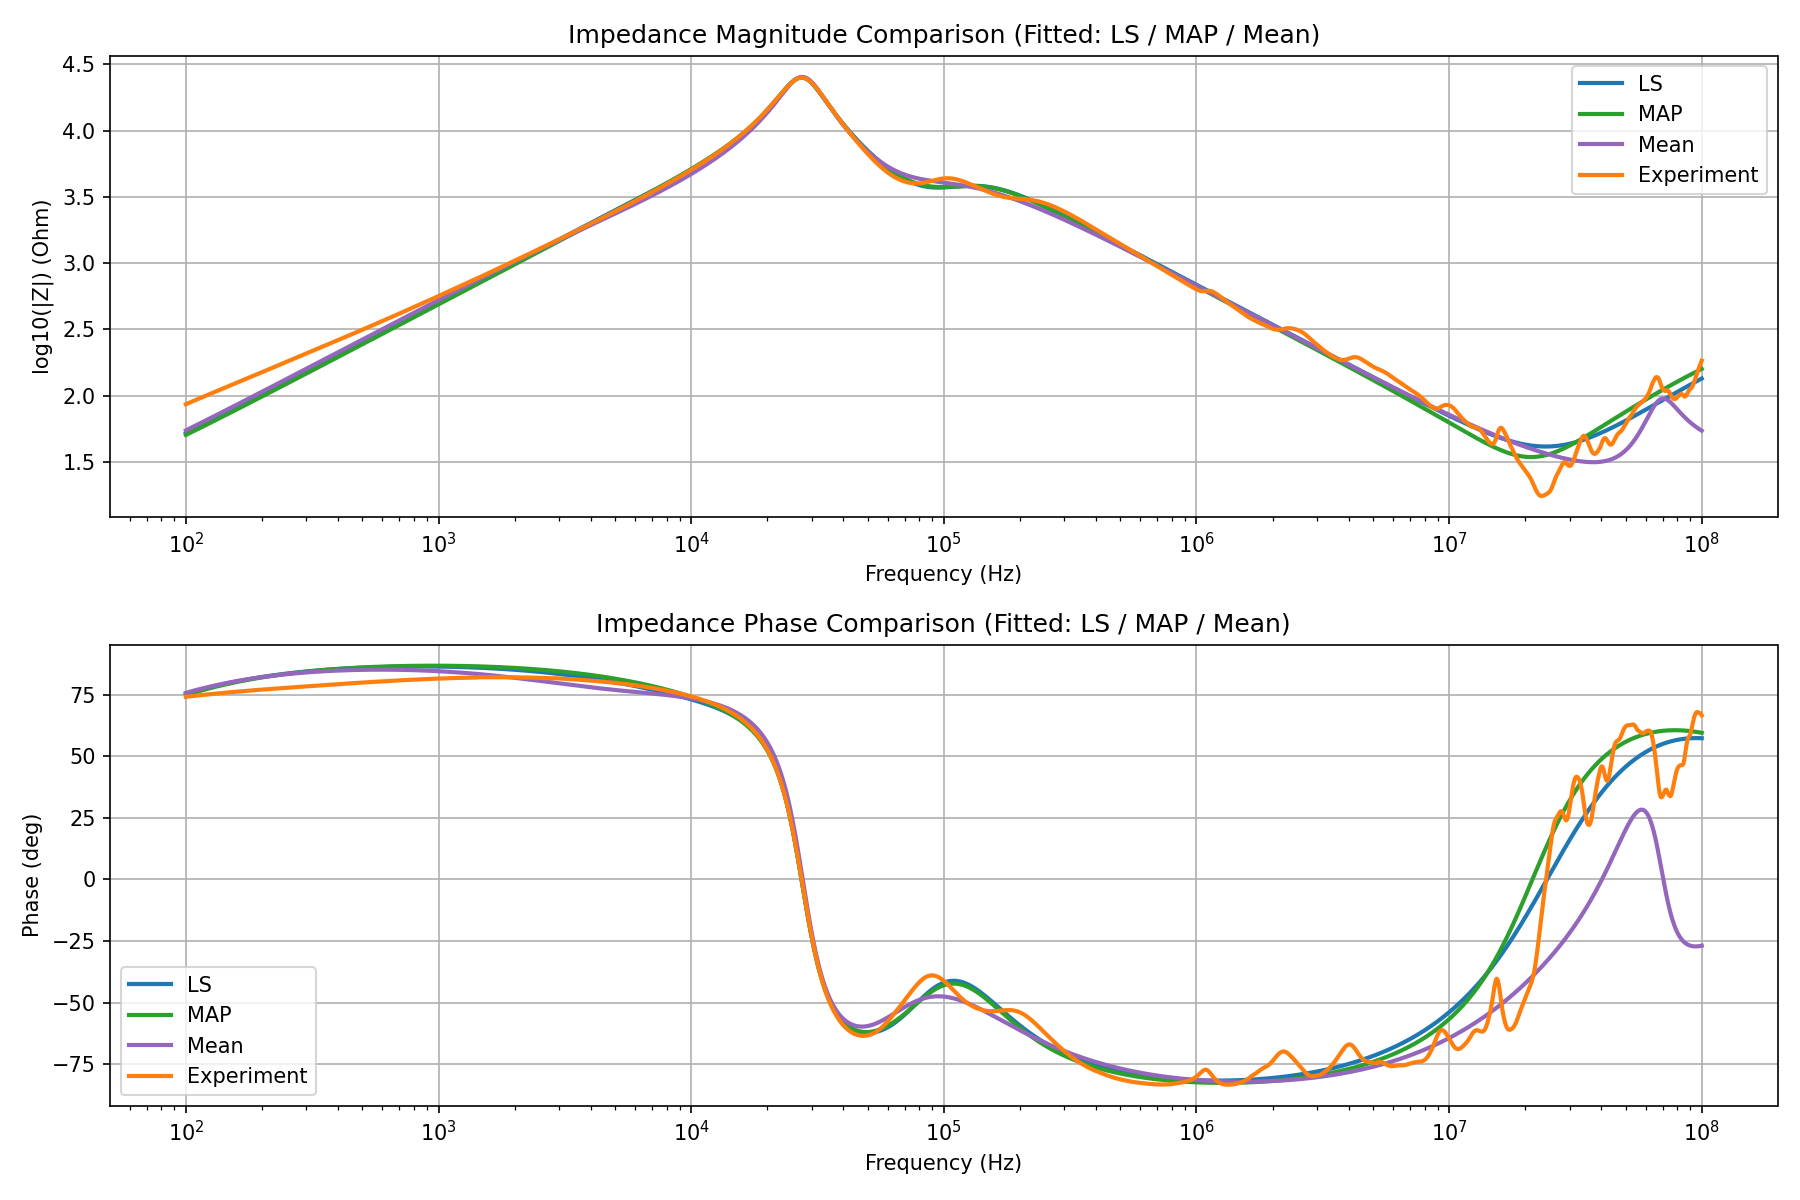
\includegraphics[width=0.82\linewidth]{fig_nuts_fit.png}
    \caption{Comparison of impedance magnitude and phase between least-squares (LS), maximum a posteriori (MAP), and posterior mean estimates obtained via NUTS sampling, against experimental measurements. The close agreement indicates that the LS solution lies near the posterior optimum, suggesting that the remaining fitting error is not due to optimization deficiency.}
    \label{fig:nuts_fit}
\end{figure}

Quantitatively, the raw-space metrics remain invariant to numerical precision following the Bayesian refinement phase, with $SSE_{\text{raw}} = 5.44654 \times 10^7$ and $RMSE_{\text{raw}} = 130.872$ for $n = 3180$. The objective costs for the top-ranking candidates are tightly clustered at $1528.3$, confirming that the identified parameters reside in a stable, high-quality region of the loss landscape. Despite a significant increase in computational effort—where the Bayesian sampling stage required $2210.610$ s compared to the $7.996$ s required by the proposed deterministic pipeline—no material improvement in fitting accuracy was observed. These findings reinforce the conclusion that the remaining residuals, particularly the localized UHF phase peaks, originate from structural constraints within the current grey-box formulation rather than an inadequately explored objective space.

\subsection{Ablation Study and Robustness Analysis}
The ablation study decomposes the proposed pipeline to evaluate the individual contributions of analytic initialization, differential evolution (DE) global search, least-squares (LS) refinement, log-bounds scaling, Re/Im residual balancing, frequency weighting, and the $soft\_l1$ robust loss. Five variants—LS-only, DE-only, No-Weights, No-Scaling, and GA+LS—are compared using a layer-by-layer removal strategy while maintaining identical datasets, parameter bounds, and circuit topologies. Each configuration is executed over 10 independent seeds to quantify performance via mean $\pm$ standard deviation across accuracy, computational cost, and parameter stability.

\subsubsection{Accuracy–Robustness Trade-off}
The proposed framework achieves the optimal balance between fitting accuracy and robustness. While both the "No-Weights" variant and the full pipeline yield the lowest average fitting errors, the proposed method exhibits near-zero cross-seed variance, indicating superior numerical stability. The accuracy ranking places the proposed method and the "No-Weights" variant at the top, followed by No-Scaling, LS-only, GA+LS, and DE-only. Crucially, the stability ranking distinguishes the proposed pipeline as the most repeatable method, whereas DE-only and GA+LS variants remain highly unstable. For reference, the identified solution reaches $RMSE_{\text{raw}} = 130.872$ with a total fitting time of $7.996$ s, establishing the benchmark for the following trade-off analysis.

\begin{figure}[htbp]
    \centering
    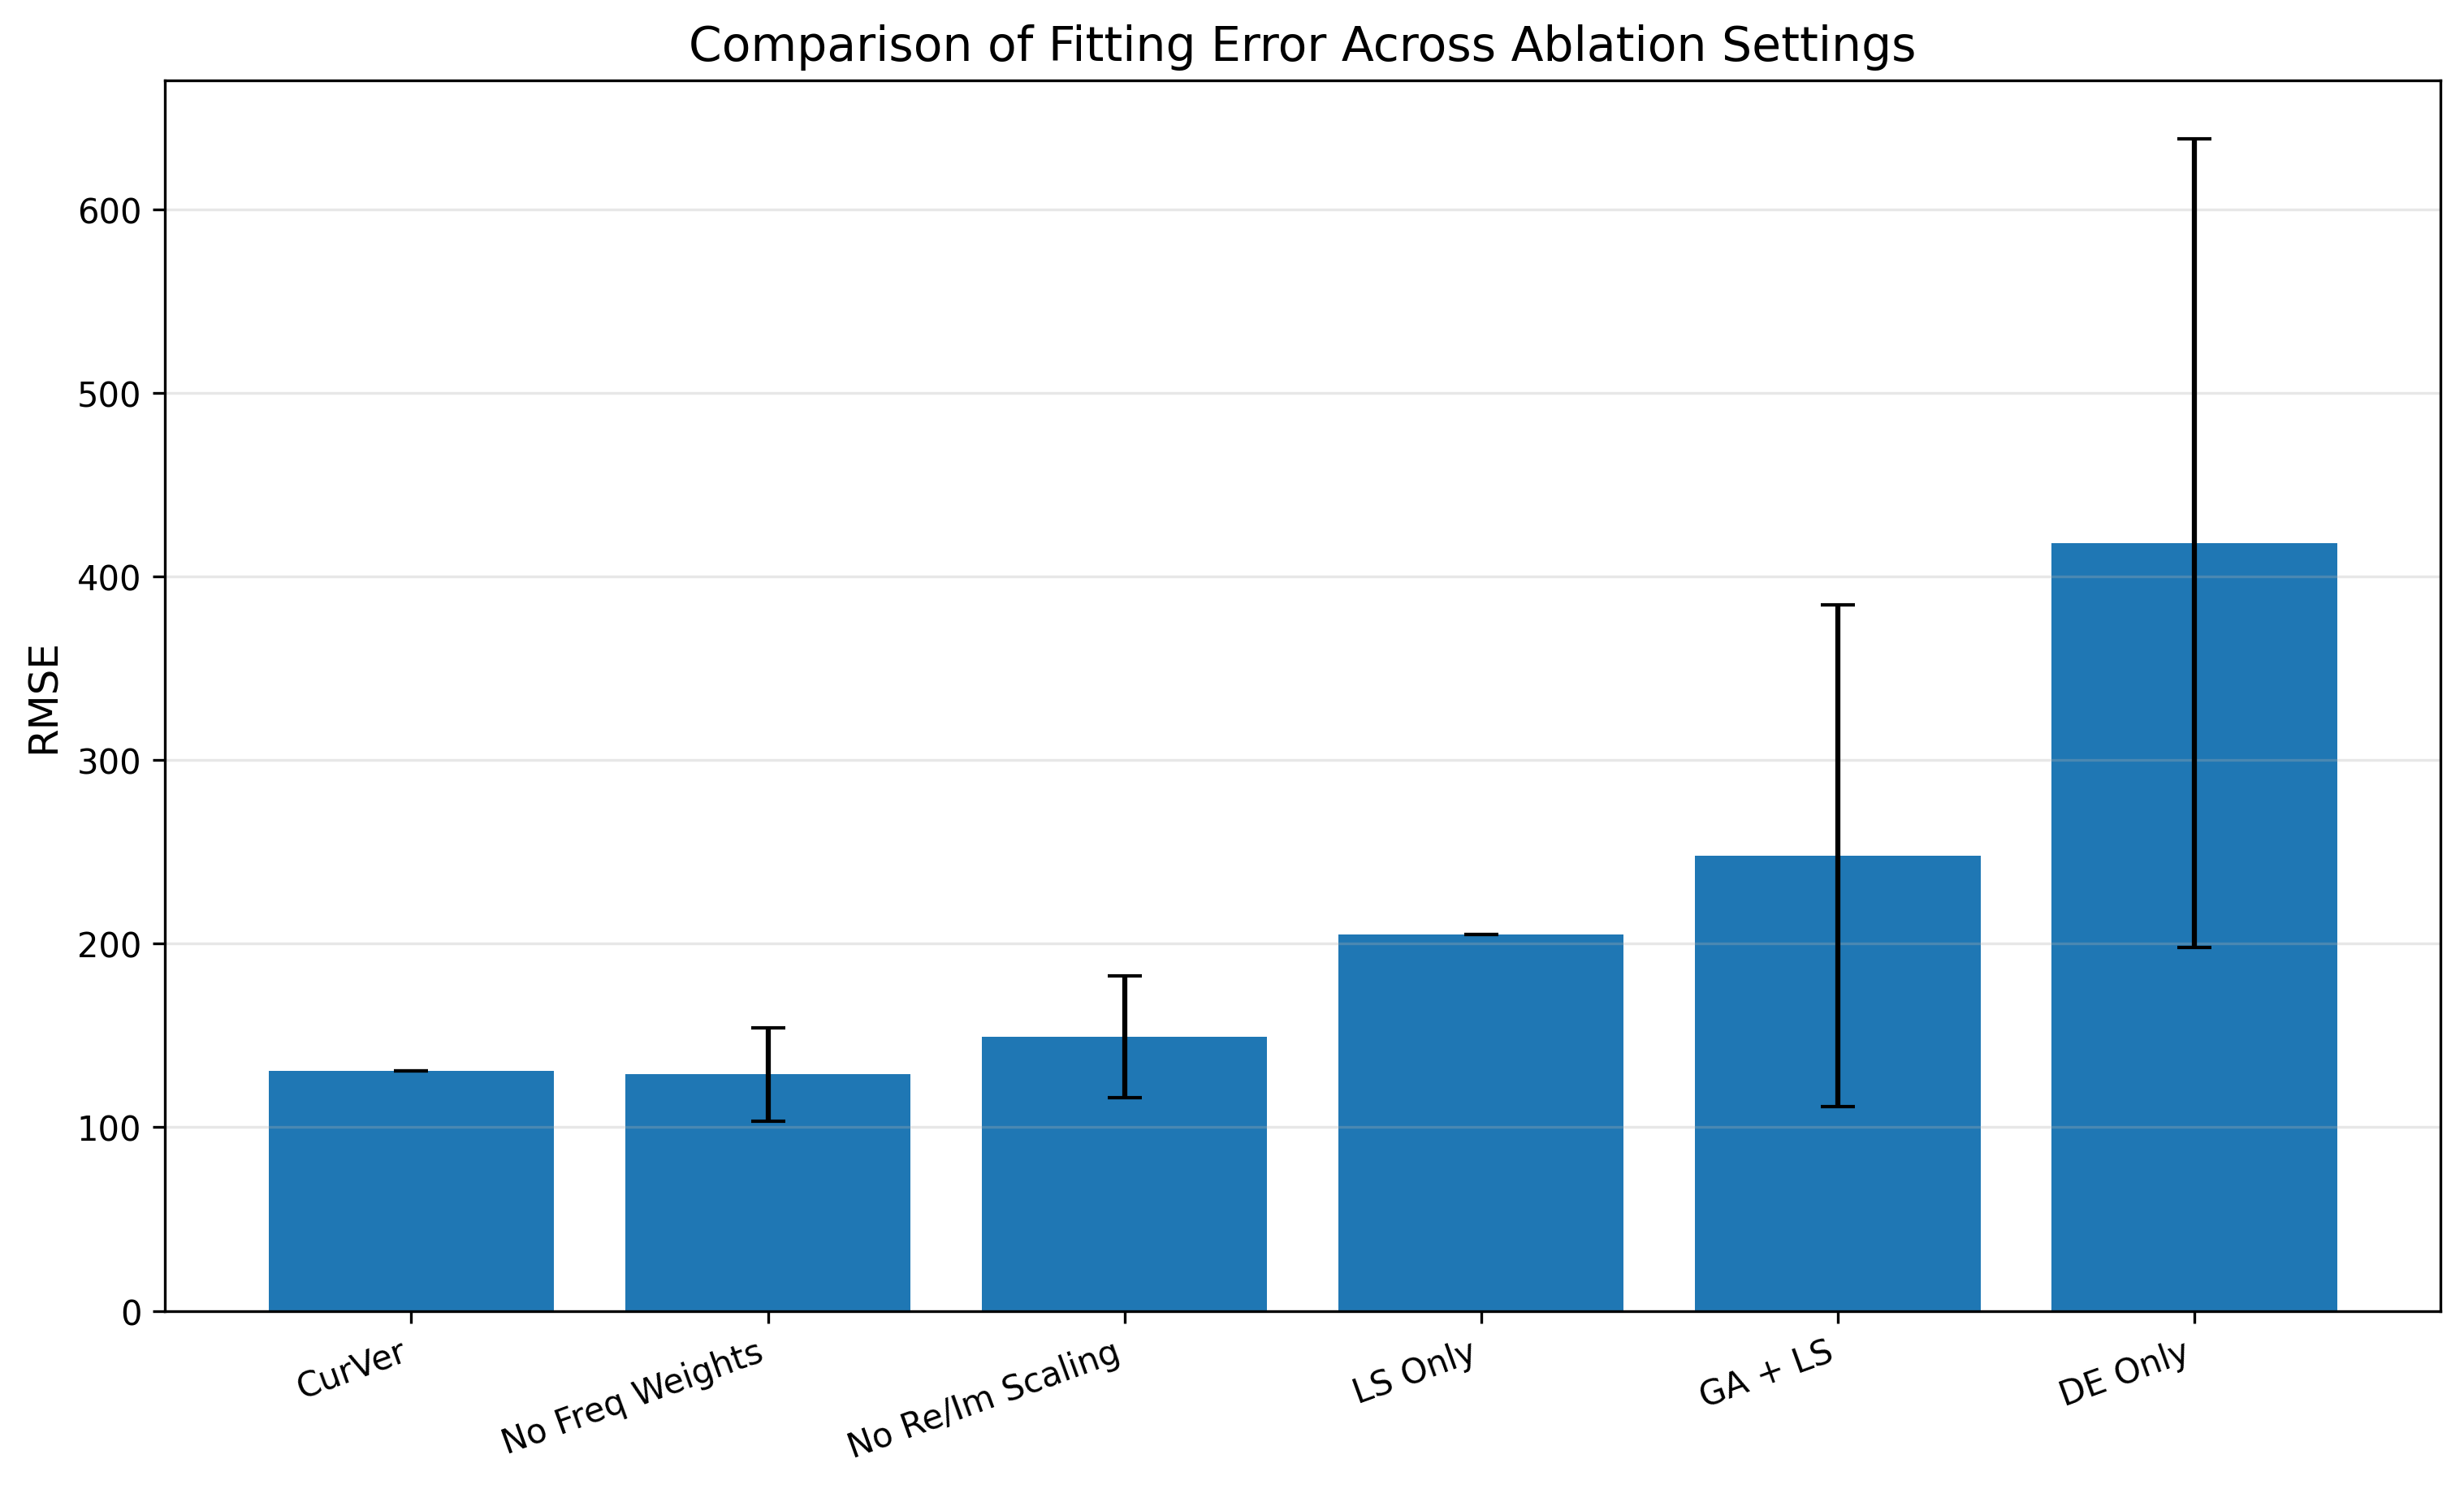
\includegraphics[width=0.82\linewidth]{fig1_rmse_bar.png}
    \caption{Comparison of fitting error across ablation settings, reported in terms of mean RMSE with error bars indicating the run-to-run variation. The current version (CurVer) achieves the lowest overall error, while removing key components of the optimization and objective design leads to varying degrees of performance degradation.}
    \label{fig:ablation_rmse}
\end{figure}

\begin{figure}[htbp]
    \centering
    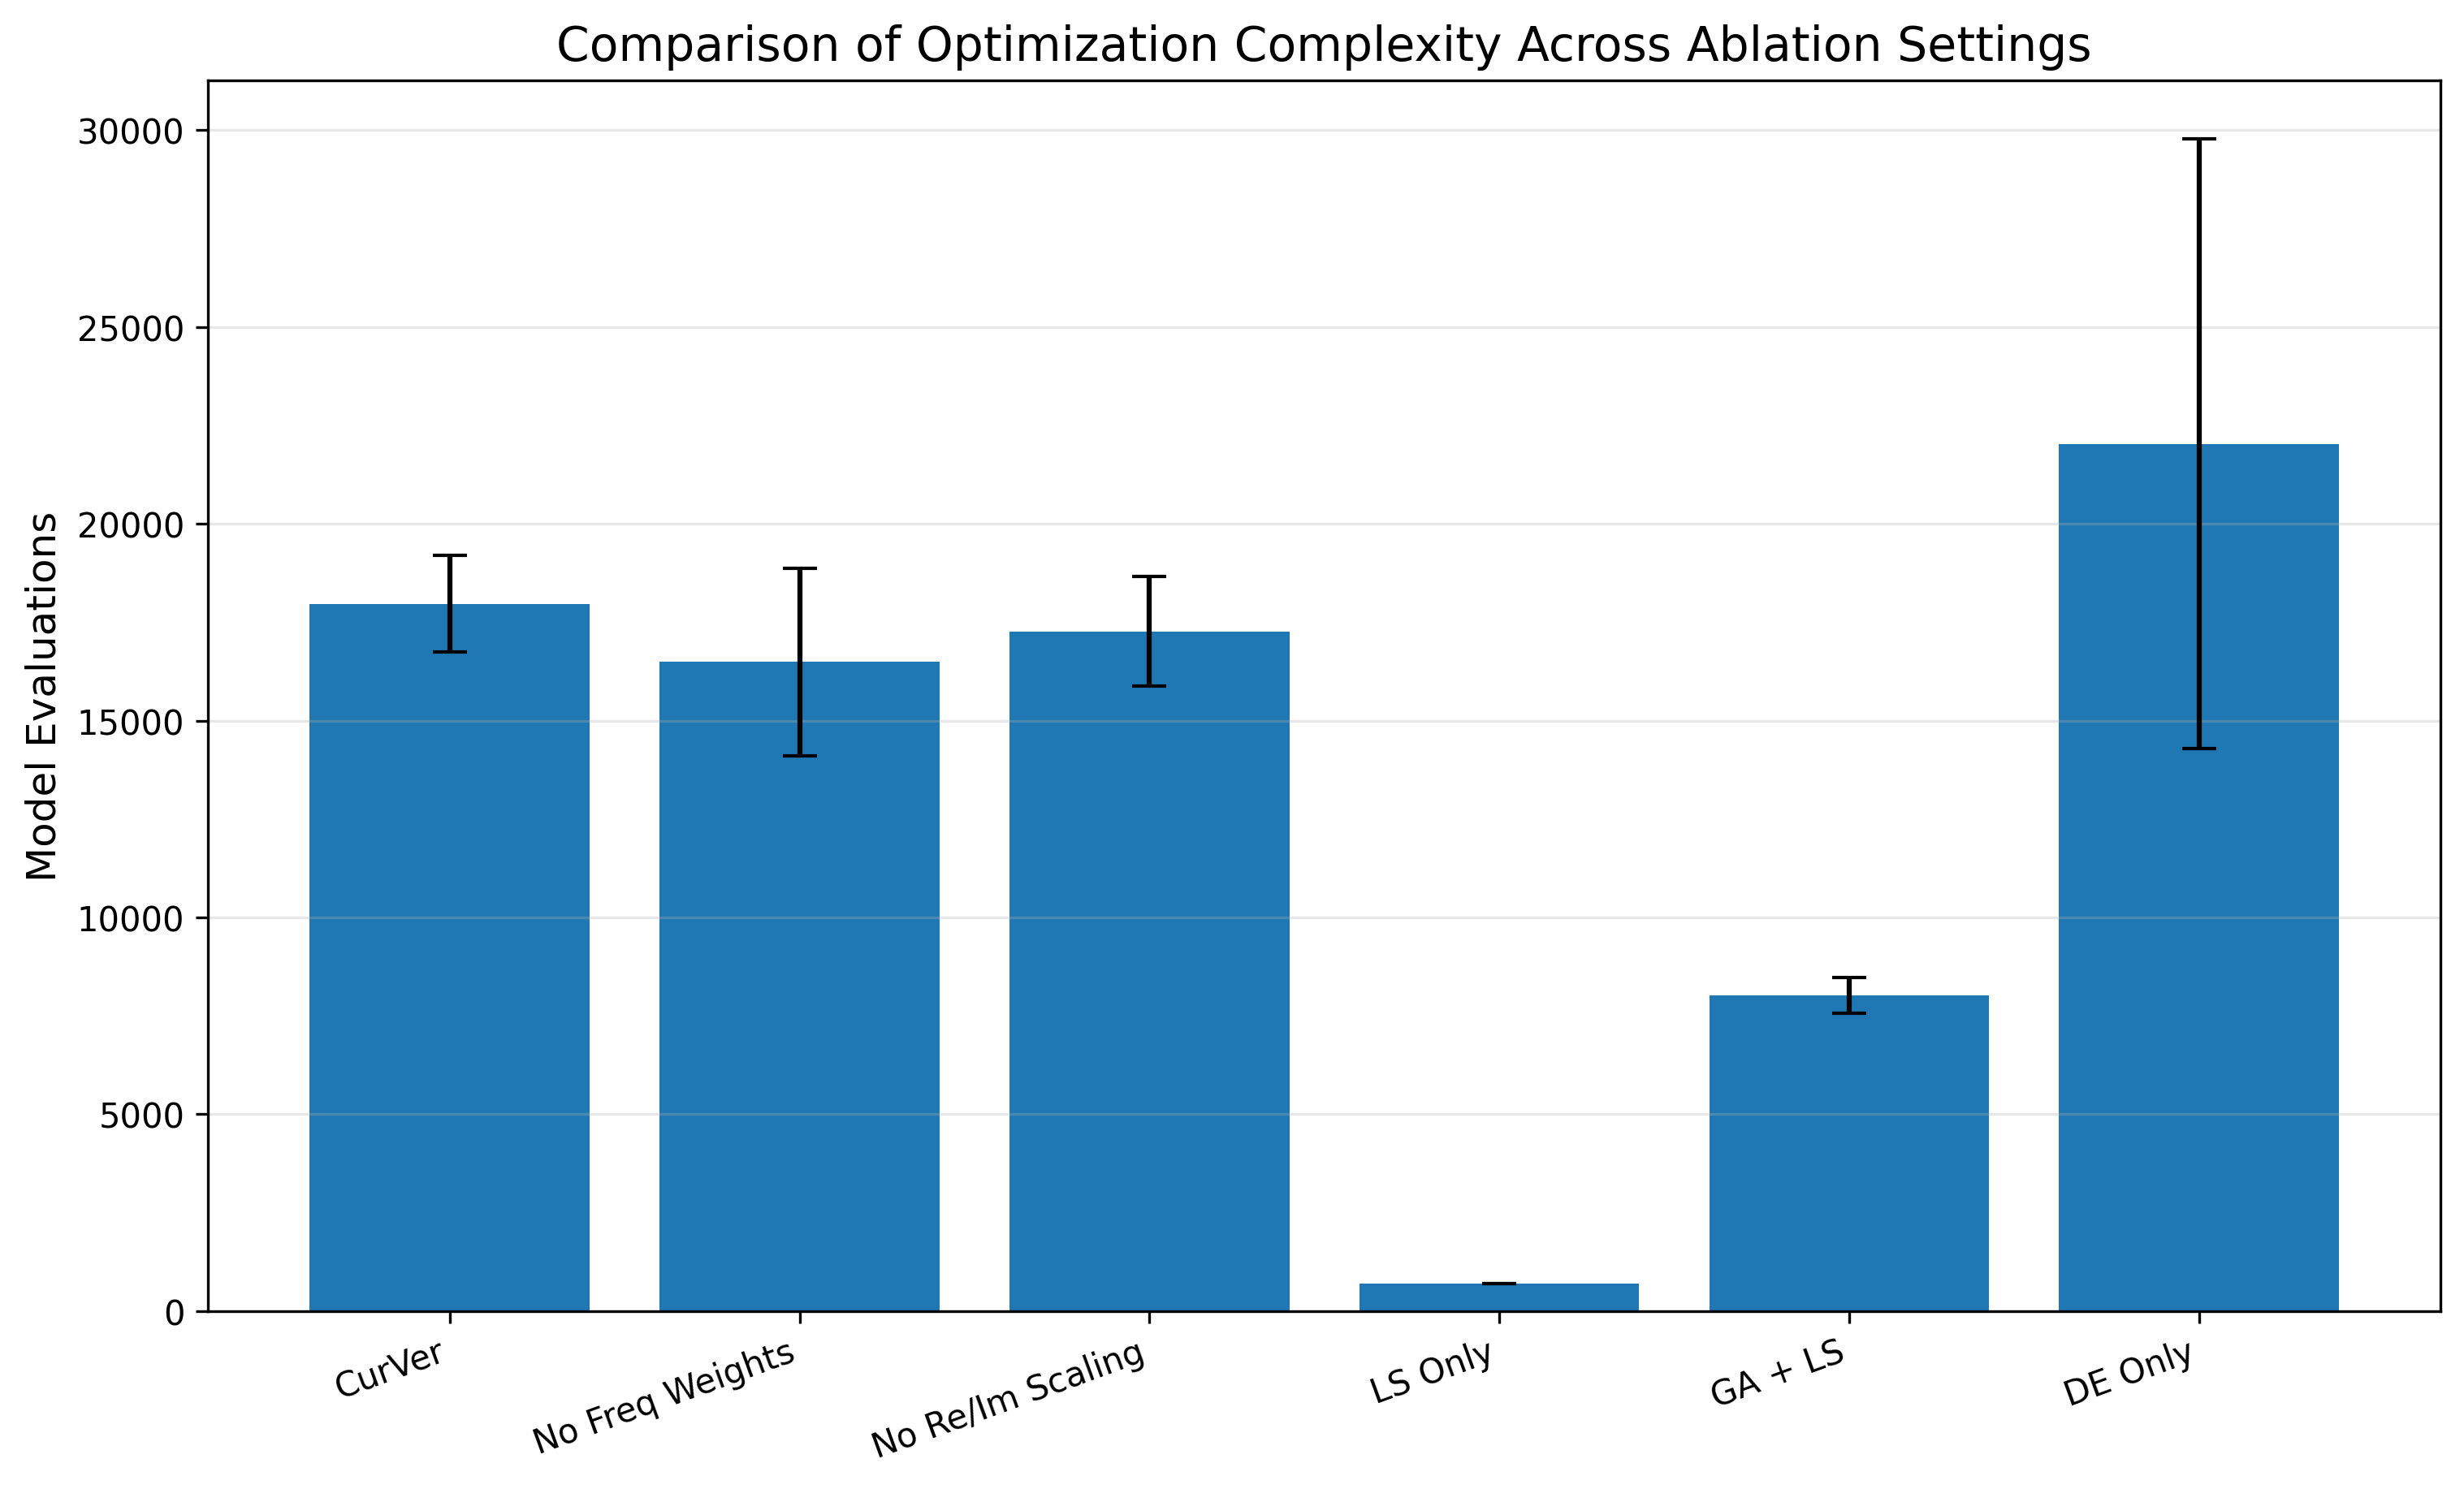
\includegraphics[width=0.82\linewidth]{fig5_model_eval_bar.png}
    \caption{Comparison of optimization complexity across ablation settings, measured by the number of model evaluations. This metric provides a hardware-independent view of computational effort and complements the wall-clock fitting time reported in Fig.~\ref{fig:ablation_time}.}
    \label{fig:ablation_complexity}
\end{figure}

\subsubsection{Optimization Framework and Strategy}
The ablation of optimization stages confirms that neither global exploration nor local refinement independently suffices for reliable identification. The LS-only approach is the most computationally efficient but converges to clearly inferior local minima. Conversely, the DE-only approach is computationally expensive yet fails to achieve acceptable accuracy, demonstrating that global search alone cannot resolve the fine-scale parameter dependencies. Although the GA+LS variant improves upon the pure global search, it remains significantly slower than the DE-based baseline without providing a commensurate gain in robustness. These results validate the necessity of the hierarchical DE+LS pipeline for navigating the objective landscape of motor impedance models.

\begin{figure}[htbp]
    \centering
    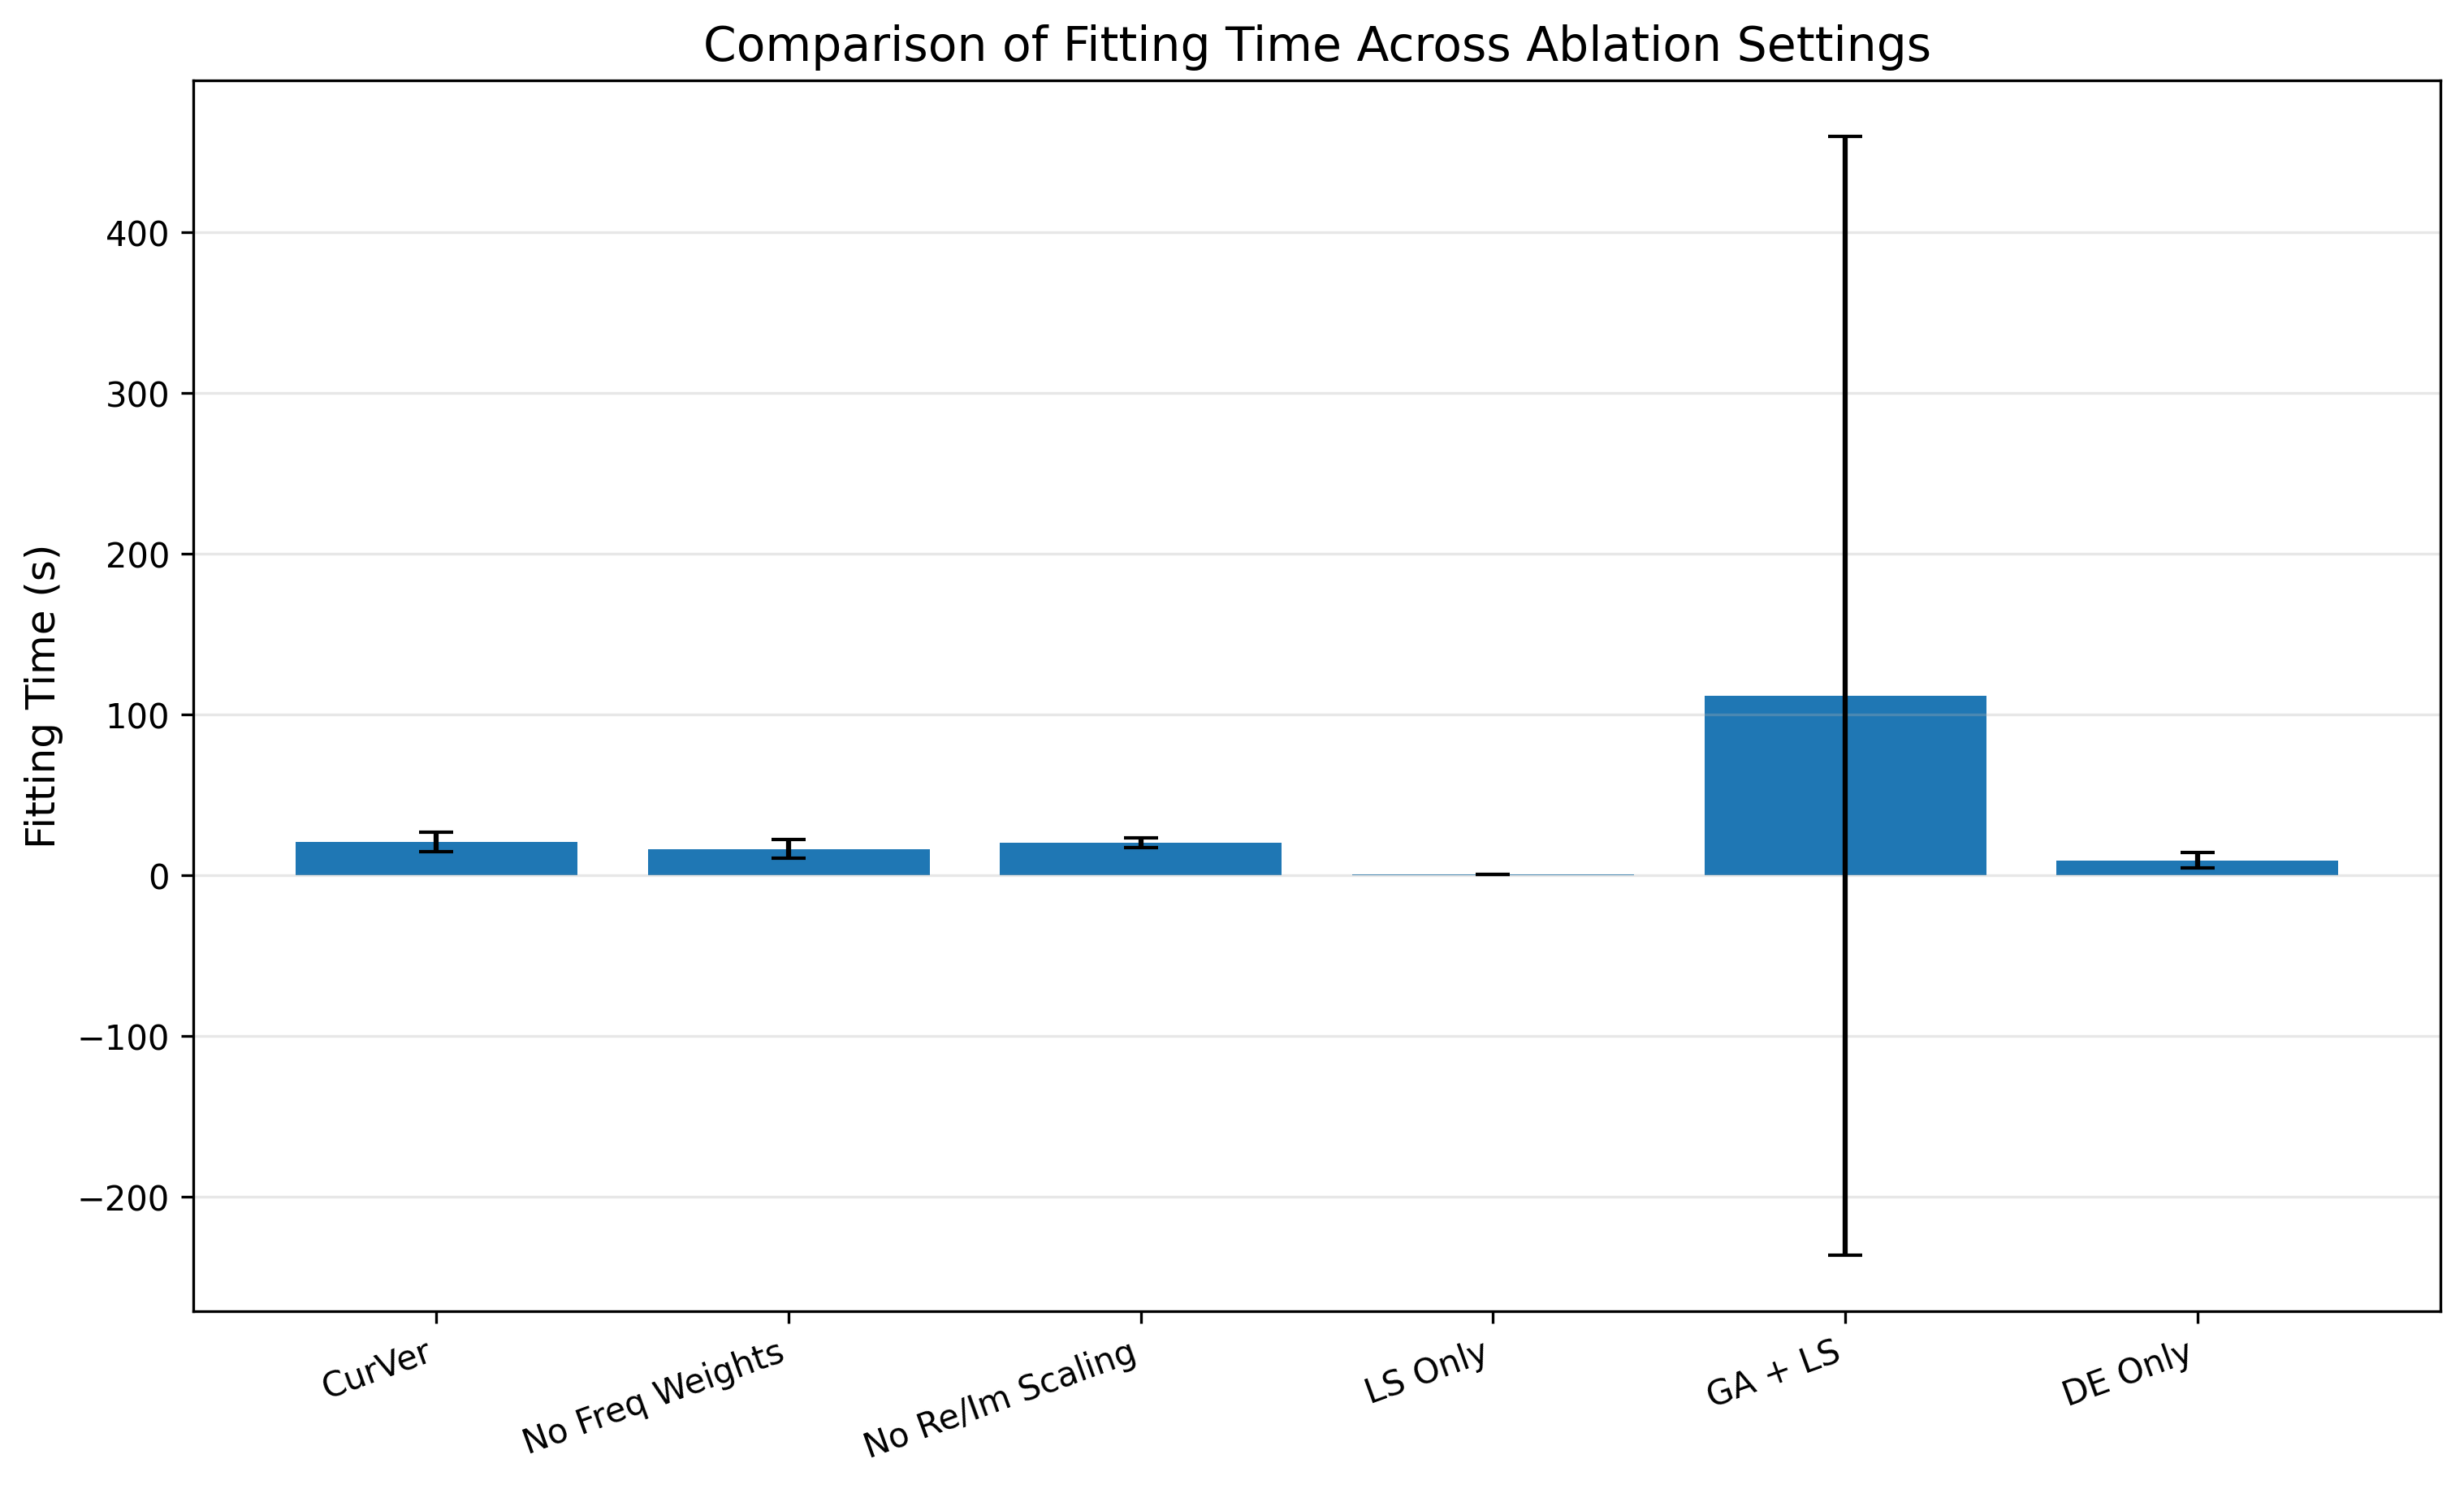
\includegraphics[width=0.82\linewidth]{fig2_tfit_bar.png}
    \caption{Comparison of fitting time across ablation settings. Error bars denote the variability across repeated runs. The results show that faster configurations, such as LS Only, achieve lower computational cost at the expense of accuracy, whereas GA + LS exhibits substantially higher time consumption and variability.}
    \label{fig:ablation_time}
\end{figure}

\begin{figure}[htbp]
    \centering
    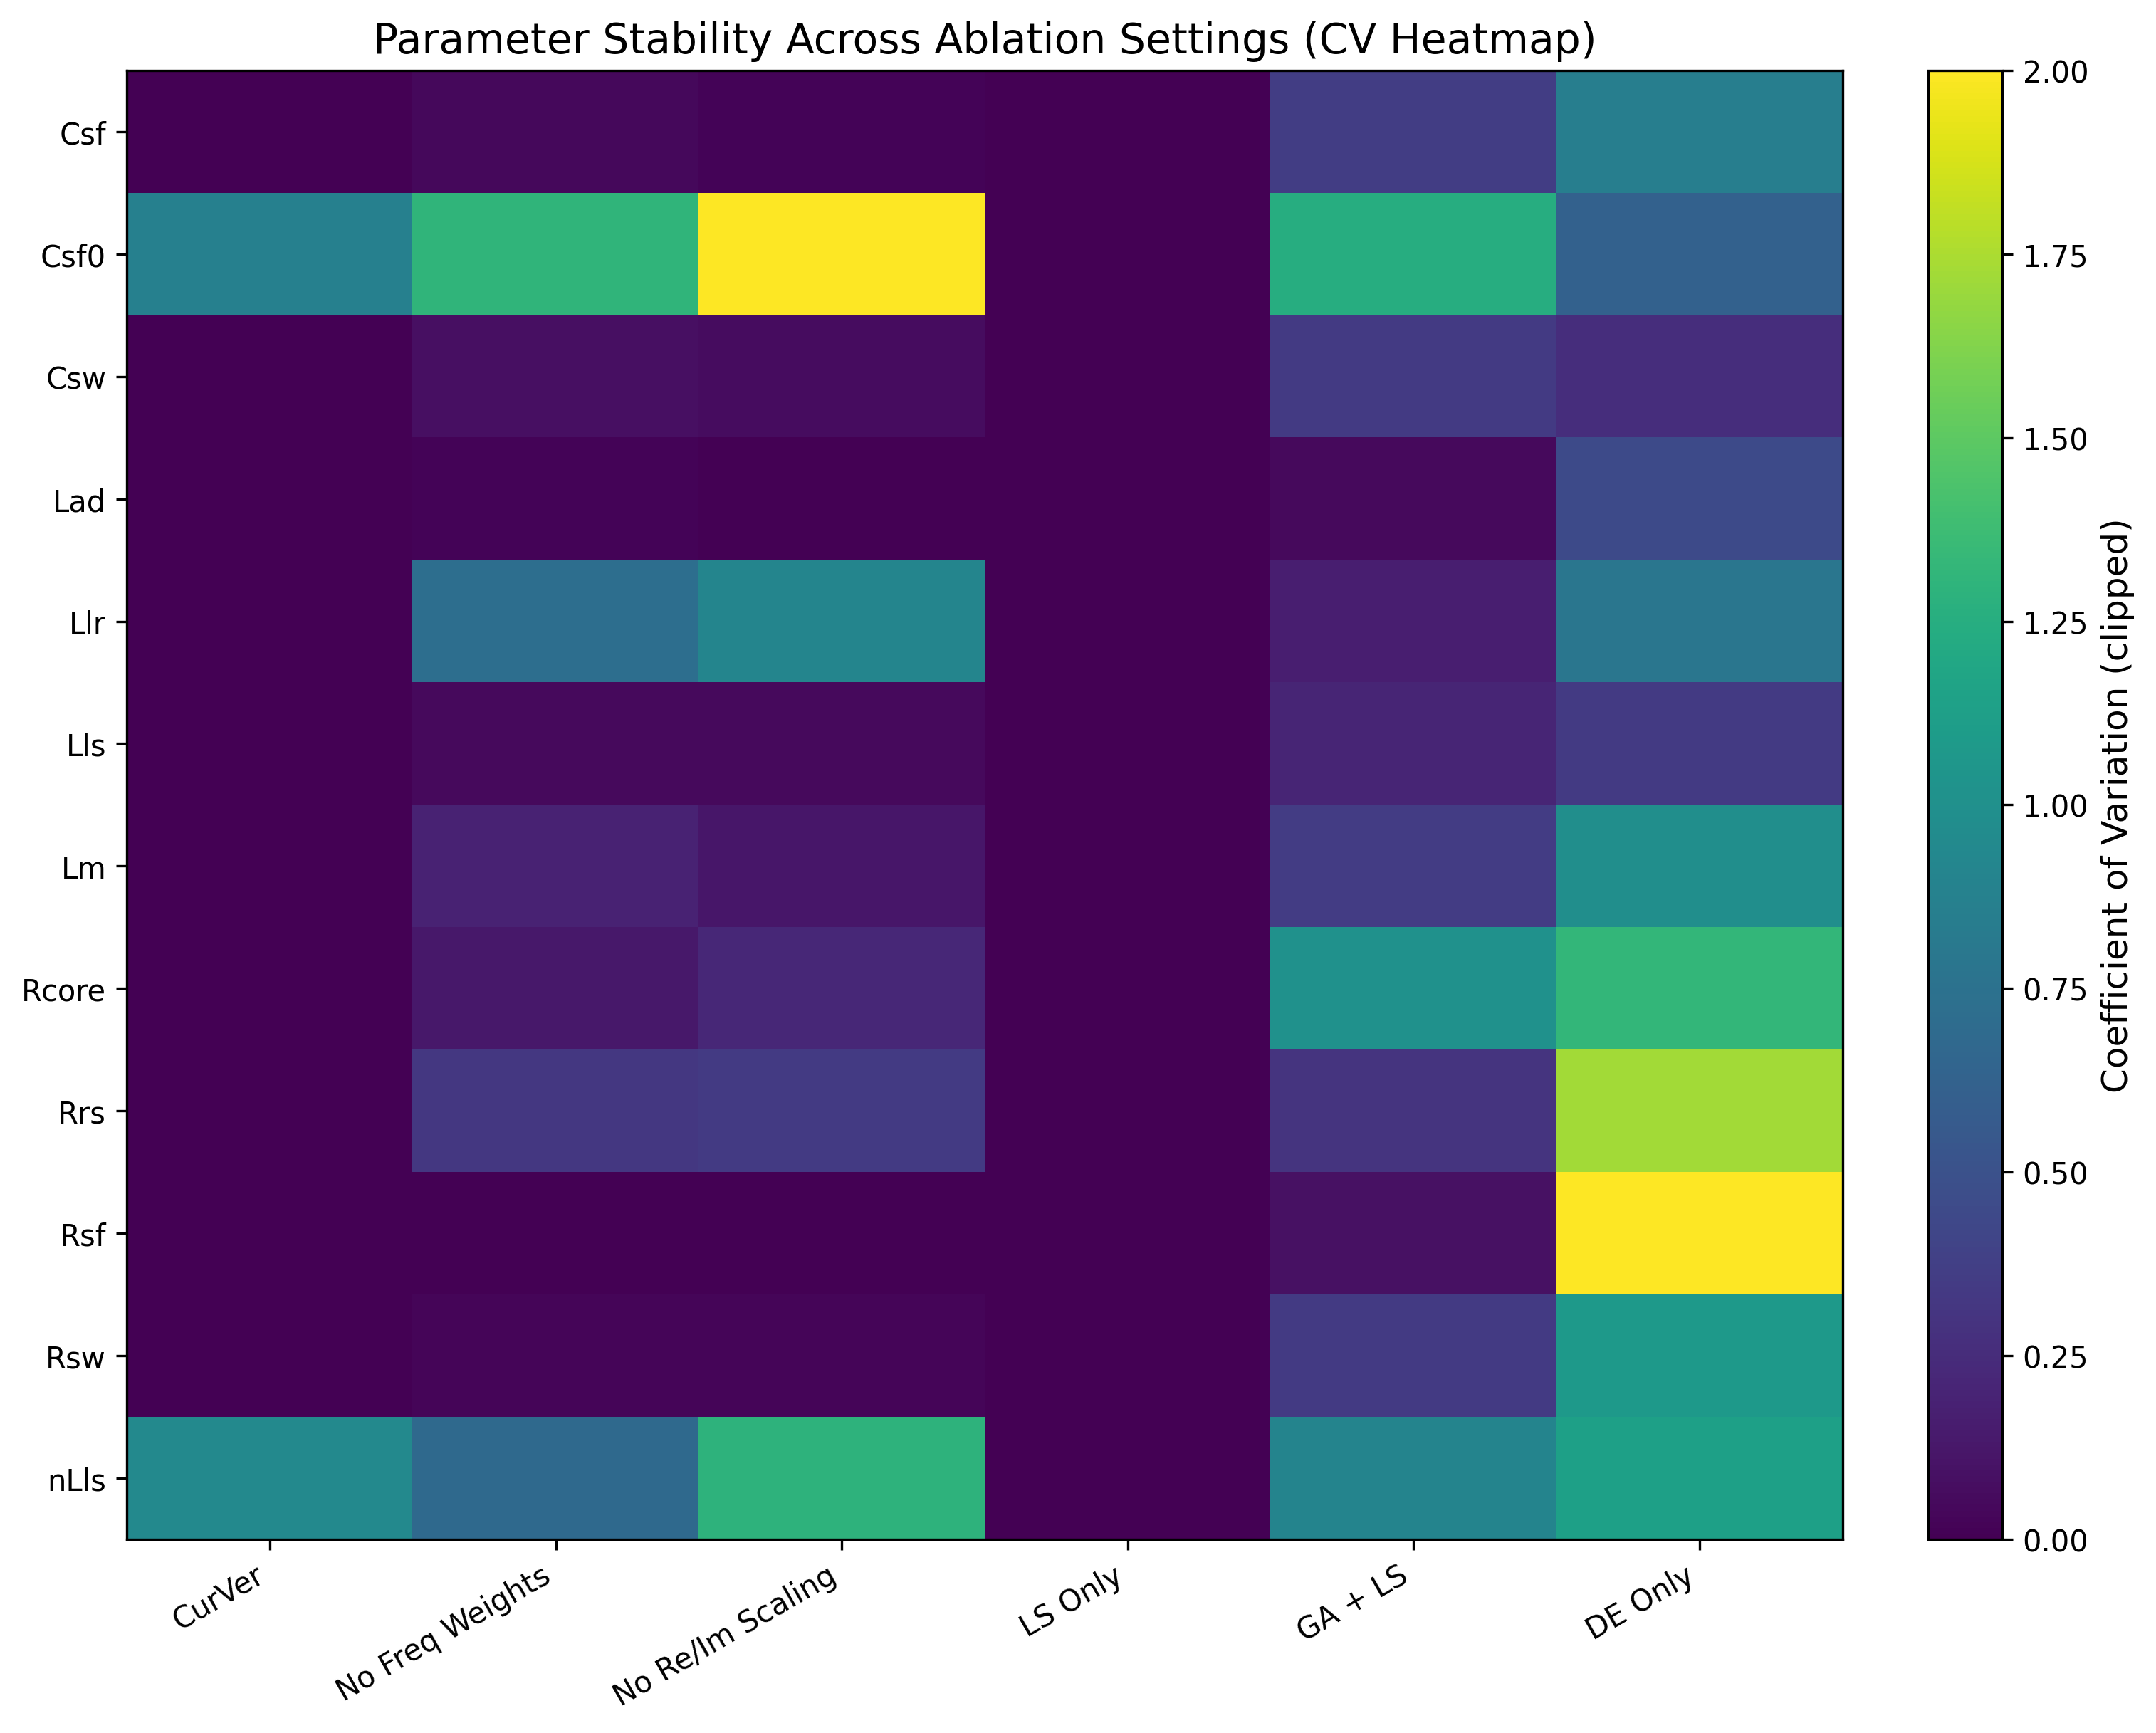
\includegraphics[width=0.82\linewidth]{fig4_param_cv_heatmap.png}
    \caption{Parameter stability across ablation settings, visualized as a heatmap of the coefficient of variation (CV) for each fitted parameter over repeated runs. Lower CV indicates greater parameter stability, while higher CV reveals increased sensitivity of the identified parameters to the corresponding ablation setting.}
    \label{fig:ablation_param_cv}
\end{figure}

\subsubsection{Role of Objective-Function Design}

Residual construction significantly influences the consistency of the identified parameters. Removing frequency weights results in a substantial increase in cross-seed variance, confirming that weighting is essential for stabilizing the fit around structurally dense regions such as resonance, anti-resonance, and high-frequency transitions. Similarly, omitting separate Re/Im scaling degrades both the fitting quality and stability, emphasizing the necessity of balancing the real and imaginary components which possess disparate magnitudes and local sensitivities. The performance of the proposed method is therefore attributable to the integration of structured residual design with a staged optimization workflow.

\subsubsection{Parameter Stability and Identifiability}

The stability analysis at the parameter level provides a dimension of validation beyond curve fitting. Under the proposed framework, the majority of circuit parameters remain stable across multiple seeds, supporting the physical consistency of the identified solution. In contrast, the DE-only and GA+LS variants exhibit excessive parameter variation, indicating poor convergence and weak identifiability. A subset of parameters, specifically $C_{sf0}$ and $nL_{ls}$, remains persistently variable across all settings, identifying them as weakly identifiable degrees of freedom characterized by strong parameter coupling. The physical locations of these two most sensitive parameters are shown in Fig.~\ref{fig:sensitive_parameters}. By localizing uncertainty to these specific terms, the proposed method enhances the overall interpretability and stability of the identified grey-box parameter set.

\begin{figure}[htbp]
    \centering
    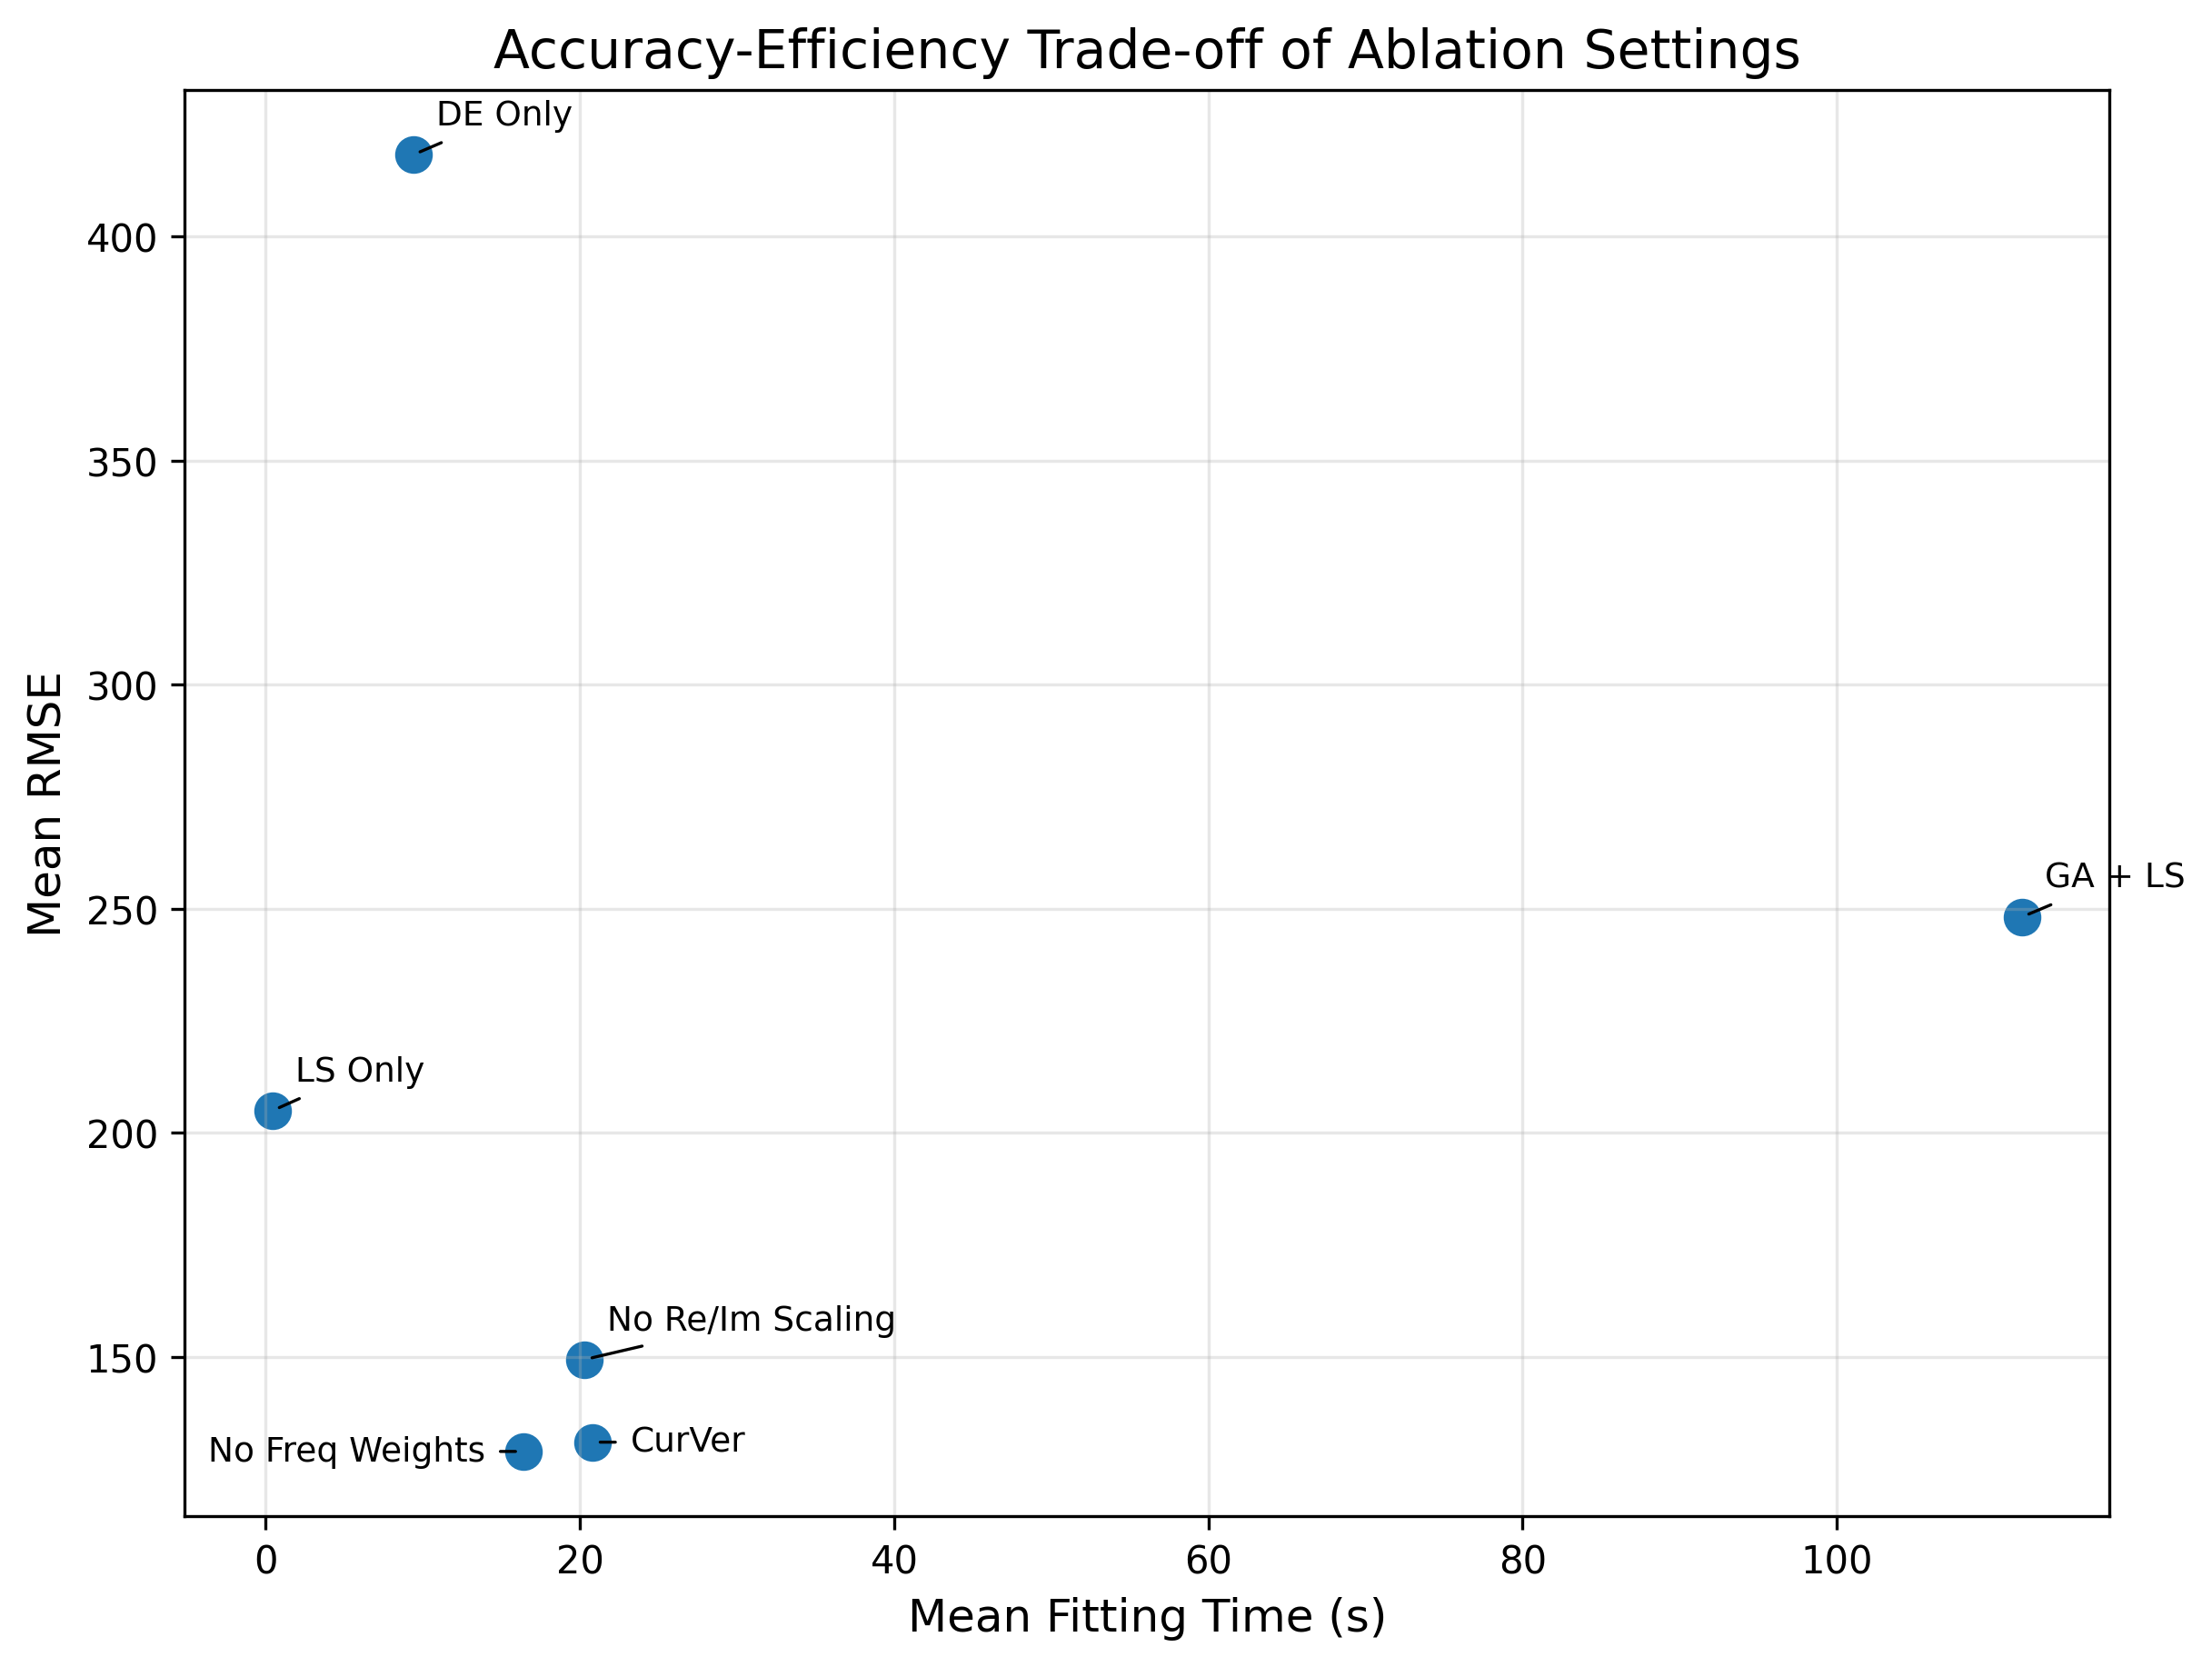
\includegraphics[width=0.82\linewidth]{fig3_rmse_vs_time.png}
    \caption{Accuracy-efficiency trade-off of different ablation settings, shown as mean RMSE versus mean fitting time. This summary view highlights the relative positioning of each setting in terms of solution quality and computational cost, showing that this method attains a favorable balance compared with the ablated alternatives.}
    \label{fig:ablation_tradeoff}
\end{figure}

\begin{figure}[htbp]
    \centering
    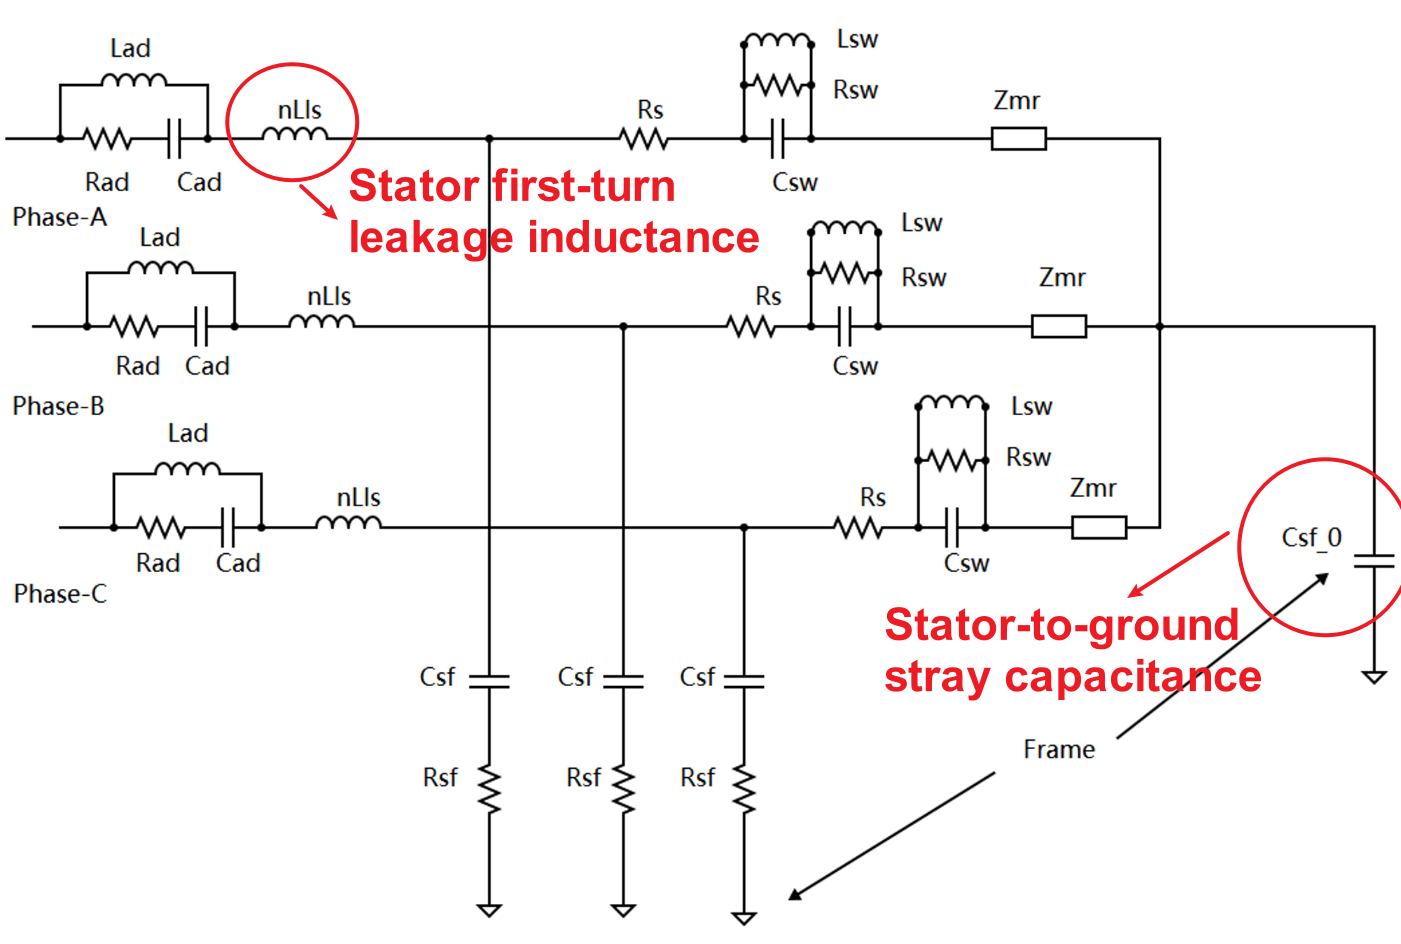
\includegraphics[width=0.82\linewidth]{Add2.png}
    \caption{Locations of the first-turn leakage inductance branch $nL_{ls}$ and the equivalent stator-to-ground stray capacitance $C_{sf0}$ in the three-phase grey-box terminal model. These parameters are directly associated with high-frequency leakage and boundary-return effects, which explains their higher sensitivity in the fitting process.}
    \label{fig:sensitive_parameters}
\end{figure}

\newpage

\section{Conclusion}

This report presented the development and evaluation of a grey-box impedance modeling workflow for induction-machine terminal impedance over the frequency range from $10^2$ to $10^8$~Hz. The project combined measured impedance-spectrum analysis, analytical parameter initialization, baseline grey-box circuit modeling, and hybrid global-to-local optimization to obtain an interpretable wideband terminal model for EMC-oriented analysis.

The baseline model captured the dominant low- and mid-frequency impedance characteristics, including the main resonance and anti-resonance behavior. In the ultra-high-frequency range near $10^{7}$--$10^{8}$~Hz, the measured response showed a phase rise and magnitude recovery that required additional high-frequency structural flexibility. A port-side resonant branch was therefore introduced as a boundary-aware equivalent extension, improving the full-band representation while preserving the physical interpretability of the grey-box model.

The validation results, residual-structure diagnosis, and ablation studies confirmed the importance of the combined identification workflow, including spectral feature extraction, analytical initialization, frequency-dependent residual weighting, separate real/imaginary scaling, and hybrid DE--LS refinement. The resulting model provides a practical basis for wideband motor terminal impedance modeling under measured boundary conditions.

The current model remains an equivalent terminal-level representation and should be further validated using additional motor samples, wiring configurations, and measurement boundary conditions. Future work may also incorporate de-embedding procedures and system-level motor-drive validation to clarify the physical origin and practical impact of the ultra-high-frequency response.

\clearpage
\addcontentsline{toc}{section}{References}
\bibliographystyle{IEEEtran}
\bibliography{references}

\end{document}